\chapter{Phân tích và thiết kế hệ thống}
\label{chap:analysis-design}

\section{Sơ đồ ca sử dụng (Use Case Diagram)}
\subsection{Giới thiệu sơ đồ ca sử dụng}
Sơ đồ ca sử dụng mô tả mối quan hệ tương tác giữa các tác nhân bên ngoài (người dùng, quản trị viên, các dịch vụ tích hợp) và tác nhân hệ thống chạy ngầm với các chức năng cốt lõi của trợ lý ảo MiniClaw. Cách biểu diễn này tập trung vào mục tiêu người dùng và ranh giới hệ thống, không đi vào chi tiết thuật toán xử lý bên trong.

\subsection{Các tác nhân trong hệ thống}
Hệ thống phân tách các thực thể tương tác thành ba nhóm vai trò chính, hệ thống và dịch vụ như sau:
\begin{itemize}
  \item \textbf{Người dùng (User - Tác nhân chính):} Là thực thể tương tác chính với trợ lý ảo thông qua giao diện Telegram. Người dùng gửi yêu cầu bằng ngôn ngữ tự nhiên để trò chuyện, thiết lập nhắc nhở, đồng bộ lịch trình, quản lý thư/công việc và tham gia kiểm duyệt quy trình làm việc (HITL).
  \item \textbf{Quản trị viên (Admin - Tác nhân chính):} Là nhà phát triển hoặc người vận hành hệ thống, thực hiện cài đặt, cấu hình biến môi trường, định cấu hình danh sách an toàn (allow-list) và khởi tạo ứng dụng qua giao diện CLI.
  \item \textbf{Tiến trình nền (Daemon - Tác nhân hệ thống):} Là tiến trình chạy ngầm liên tục trên máy chủ cá nhân để điều phối bộ lập lịch sự kiện, giám sát tệp tin kỹ năng để nạp động công cụ mới và kích hoạt kiểm tra nén ngữ cảnh định kỳ.
  \item \textbf{Dịch vụ Lịch trình (Calendar Service - Tác nhân dịch vụ):} Giao tiếp với API ngoài (Google Calendar, Lark Calendar) để đồng bộ sự kiện lịch biểu.
  \item \textbf{Dịch vụ Thư điện tử (Mail Service - Tác nhân dịch vụ):} Giao tiếp với API ngoài (Gmail, Lark Mail) để quản lý thư tín.
  \item \textbf{Dịch vụ Công việc (Task Service - Tác nhân dịch vụ):} Giao tiếp với API ngoài (Google Tasks, Lark Tasks) để cập nhật và đồng bộ danh sách tác vụ thường nhật.
\end{itemize}

\subsection{Các ca sử dụng chính}
Các ca sử dụng chính của hệ thống MiniClaw được phân chia theo hai trụ cột nghiệp vụ cốt lõi của đề tài (quản lý lịch trình, công việc hàng ngày) kết hợp cùng cơ chế quản trị và tự động hóa tác nhân.

\begin{center}
  \resizebox{\textwidth}{!}{
  \begin{tikzpicture}[
      % --- GLOBAL STYLES & SEMANTIC COLORS (MONOCHROME) ---
      every node/.style={font=\small},
      sys-neutral/.style={rectangle, draw=black!80, fill=gray!20, thick, rounded corners=2pt, align=center},
      sys-client/.style={rectangle, draw=black!80, fill=gray!10, thick, rounded corners=2pt, align=center},
      sys-core/.style={rectangle, draw=black!80, fill=white, thick, rounded corners=2pt, align=center},
      sys-data/.style={rectangle, draw=black!80, fill=gray!10, thick, rounded corners=2pt, align=center},
      sys-alert/.style={rectangle, draw=black!100, fill=gray!20, double, thick, rounded corners=2pt, align=center},
      %
      uc/.style={minimum width=6.4cm, minimum height=0.75cm, text width=6.4cm, align=center, inner sep=2pt},
      actor/.style={minimum width=2.8cm, minimum height=1.1cm, text width=2.6cm, align=center, inner sep=3pt},
      line/.style={thick, draw=black!70}
  ]
    %
    % 1. System Boundary
    \draw[thick, draw=black!80, fill=gray!5, rounded corners=4pt] (-3.8, 1.0) rectangle (3.8, -10.4);
    \node[font=\scriptsize\itshape, anchor=south] at (0, 1.02) {«system»};
    \node[font=\bfseries\small, anchor=north] at (0, 0.8) {Hệ thống MiniClaw};
    %
    % 2. Use Cases 
    \node[sys-core, uc] (uc1) at (0, -0.4) {UC-01: Trò chuyện tự nhiên};
    \node[sys-core, uc] (uc2) at (0, -1.5) {UC-02: Lập lịch \& cập nhật sự kiện};
    \node[sys-core, uc] (uc3) at (0, -2.6) {UC-03: Thiết lập nhắc nhở cục bộ};
    \node[sys-core, uc] (uc4) at (0, -3.7) {UC-04: Kích hoạt nhắc nhở};
    \node[sys-core, uc] (uc5) at (0, -4.8) {UC-05: Quản lý thư điện tử};
    \node[sys-core, uc] (uc6) at (0, -5.9) {UC-06: Quản lý công việc};
    \node[sys-alert, uc] (uc7) at (0, -7.0) {UC-07: Duyệt quy trình (HITL)};
    \node[sys-core, uc] (uc8) at (0, -8.1) {UC-08: Nạp động quy trình mới};
    \node[sys-core, uc] (uc9) at (0, -9.2) {UC-09: Khởi tạo hệ thống CLI};
    %
    % 3. Primary Actors
    \node[sys-client, actor] (user) at (-6.8, -3.7) {Người dùng\protect\\(User)};
    \node[font=\scriptsize\itshape, above=2pt] at (user.north) {«actor»};
    \node[sys-client, actor] (admin) at (-6.8, -9.2) {Quản trị viên\protect\\(Admin)};
    \node[font=\scriptsize\itshape, above=2pt] at (admin.north) {«actor»};
    %
    % 4. Secondary Actors (stereotype as separate node above each box)
    \node[sys-data, actor] (calendar) at (6.8, -1.0) {Dịch vụ Lịch trình\protect\\(Calendar API)};
    \node[font=\scriptsize\itshape, above=2pt] at (calendar.north) {«service»};
    \node[sys-data, actor] (mail) at (6.8, -3.4) {Dịch vụ Thư điện tử\protect\\(Mail API)};
    \node[font=\scriptsize\itshape, above=2pt] at (mail.north) {«service»};
    \node[sys-data, actor] (task) at (6.8, -5.8) {Dịch vụ Công việc\protect\\(Task API)};
    \node[font=\scriptsize\itshape, above=2pt] at (task.north) {«service»};
    \node[sys-neutral, actor] (daemon) at (6.8, -8.2) {Tiến trình nền\protect\\(Daemon)};
    \node[font=\scriptsize\itshape, above=2pt] at (daemon.north) {«daemon»};
    %
    % 5. Link User
    \draw[line] (user.east) -- (uc1.west);
    \draw[line] (user.east) -- (uc2.west);
    \draw[line] (user.east) -- (uc3.west);
    \draw[line] (user.east) -- (uc5.west);
    \draw[line] (user.east) -- (uc6.west);
    \draw[line] (user.east) -- (uc7.west);
    %
    % 6. Link Admin
    \draw[line] (admin.east) -- (uc9.west);
    %
    % 7. Link Services
    \draw[line] (uc2.east) -- (calendar.west);
    \draw[line] (uc5.east) -- (mail.west);
    \draw[line] (uc6.east) -- (task.west);
    %
    % 8. Link Daemon
    \draw[line] (daemon.west) -- (uc4.east);
    \draw[line] (daemon.west) -- (uc7.east);
    \draw[line] (daemon.west) -- (uc8.east);
  \end{tikzpicture}
  }
  
  \captionof{figure}{\emph{Sơ đồ ca sử dụng tổng thể của hệ thống MiniClaw.}}
  \label{fig:use-case-diagram}
\end{center}



Phân tích sơ đồ Hình \ref{fig:use-case-diagram} cho thấy tính phân tách rõ ràng giữa các tác nhân bên ngoài và các tiến trình tự động của hệ thống. Bằng cách đưa \texttt{Daemon} làm tác nhân hệ thống phụ trách kích hoạt (trigger) các tác vụ chạy ngầm như \texttt{UC-04}, \texttt{UC-07} và \texttt{UC-08}, MiniClaw duy trì tính tự trị cao mà không cần sự can thiệp trực tiếp từ người dùng. Sự trừu tượng hóa các tác nhân dịch vụ (\texttt{Calendar Service}, \texttt{Mail Service}, \texttt{Task Service}) giúp cô lập logic nghiệp vụ của trợ lý ảo khỏi các nhà cung cấp cụ thể (Google Workspace, Lark Suite), từ đó tăng khả năng bảo trì và mở rộng hệ thống sau này.

\subsection{Đặc tả ca sử dụng chi tiết (Use Case Specification)}
Bảng đặc tả dưới đây trình bày luồng nghiệp vụ chính, điều kiện tiên quyết, hậu điều kiện và các ngoại lệ cho toàn bộ chín ca sử dụng của hệ thống MiniClaw.

% ---- UC-01 ----
\subsubsection{UC-01: Trò chuyện tự nhiên}
\label{subsec:spec-uc01}
\renewcommand{\arraystretch}{1.4}
\begin{longtable}{|>{\bfseries}p{3.5cm}|p{10.5cm}|}
  \caption{\emph{Đặc tả UC-01: Trò chuyện tự nhiên.}} \label{tab:spec-uc01} \\
  \hline
  Mã use case      & UC-01 \\ \hline
  Tên use case     & Trò chuyện tự nhiên \\ \hline
  Mô tả            & Người dùng gửi tin nhắn ngôn ngữ tự nhiên qua Telegram. AgentLoop tiếp nhận, gộp tin (Message Coalescing 250ms), suy luận LLM và phản hồi. \\ \hline
  Actors           & Người dùng (User) \\ \hline
  Pre-Conditions   & Hệ thống đang chạy; người dùng trong danh sách allowlist. \\ \hline
  Post-Conditions  & Phản hồi gửi về Telegram; lịch sử hội thoại cập nhật vào bộ nhớ ngắn hạn. \\ \hline
  Main Flow        & (1) Người dùng gửi tin nhắn qua Telegram.\newline
                     (2) Telegram Bot đẩy vào MessageBus.\newline
                     (3) MessageBus gộp tin theo cửa sổ debounce 250ms.\newline
                     (4) AgentLoop nhận batch, khởi tạo vòng lặp suy luận.\newline
                     (5) LLM sinh phản hồi hoặc lệnh gọi công cụ.\newline
                     (6) Phản hồi gửi lại người dùng qua Telegram. \\ \hline
  Alternative Flow & [A1] Nhiều tin nhắn trong 250ms → gộp thành batch duy nhất.\newline
                     [A2] LLM gọi Tool → thực thi → lấy kết quả → tiếp tục suy luận. \\ \hline
  Exception        & [E1] LLM API timeout: thông báo lỗi, kết thúc vòng lặp.\newline
                     [E2] Người dùng ngoài allowlist: từ chối, không phản hồi. \\ \hline
  Business Rules   & Chỉ người dùng trong allowlist được tương tác.\newline
                     Lịch sử được nén (summarize) khi vượt ngưỡng context window. \\ \hline
\end{longtable}

% ---- UC-02 ----
\subsubsection{UC-02: Lập lịch \& cập nhật sự kiện}
\label{subsec:spec-uc02}
\renewcommand{\arraystretch}{1.4}
\begin{longtable}{|>{\bfseries}p{3.5cm}|p{10.5cm}|}
  \caption{\emph{Đặc tả UC-02: Lập lịch \& cập nhật sự kiện.}} \label{tab:spec-uc02} \\
  \hline
  Mã use case      & UC-02 \\ \hline
  Tên use case     & Lập lịch \& cập nhật sự kiện \\ \hline
  Mô tả            & Người dùng yêu cầu tạo, chỉnh sửa hoặc xóa sự kiện lịch qua ngôn ngữ tự nhiên. AgentLoop gọi Calendar Tool tích hợp với Calendar API ngoài. \\ \hline
  Actors           & Người dùng (User); Dịch vụ Lịch trình (Calendar API) \\ \hline
  Pre-Conditions   & Calendar API credentials đã cấu hình trong biến môi trường. \\ \hline
  Post-Conditions  & Sự kiện được tạo/cập nhật/xóa trên Calendar API; người dùng nhận xác nhận. \\ \hline
  Main Flow        & (1) Người dùng yêu cầu lập lịch bằng ngôn ngữ tự nhiên.\newline
                     (2) AgentLoop phân tích ý định và trích xuất thông tin sự kiện.\newline
                     (3) Gọi Calendar Tool với tham số sự kiện.\newline
                     (4) Calendar Tool giao tiếp với Calendar API (Google / Lark).\newline
                     (5) Kết quả trả về AgentLoop.\newline
                     (6) AgentLoop gửi xác nhận cho người dùng. \\ \hline
  Alternative Flow & [A1] Sự kiện trùng giờ → hỏi người dùng xác nhận ghi đè.\newline
                     [A2] Người dùng yêu cầu xem danh sách sự kiện → trả về từ API. \\ \hline
  Exception        & [E1] Calendar API lỗi/timeout: thông báo người dùng, ghi log.\newline
                     [E2] Thông tin sự kiện thiếu: yêu cầu người dùng bổ sung. \\ \hline
  Business Rules   & Chỉ thao tác trên lịch của người dùng đã xác thực qua OAuth.\newline
                     Định dạng thời gian theo múi giờ cục bộ cấu hình trong hệ thống. \\ \hline
\end{longtable}

% ---- UC-03 ----
\subsubsection{UC-03: Thiết lập nhắc nhở cục bộ}
\label{subsec:spec-uc03}
\renewcommand{\arraystretch}{1.4}
\begin{longtable}{|>{\bfseries}p{3.5cm}|p{10.5cm}|}
  \caption{\emph{Đặc tả UC-03: Thiết lập nhắc nhở cục bộ.}} \label{tab:spec-uc03} \\
  \hline
  Mã use case      & UC-03 \\ \hline
  Tên use case     & Thiết lập nhắc nhở cục bộ \\ \hline
  Mô tả            & Người dùng đặt nhắc nhở tại thời điểm cụ thể. Nhắc nhở lưu cục bộ dạng JSON và được \texttt{TaskScheduler} quản lý. \\ \hline
  Actors           & Người dùng (User) \\ \hline
  Pre-Conditions   & Hệ thống đang chạy; \texttt{TaskScheduler} đã khởi tạo. \\ \hline
  Post-Conditions  & Nhắc nhở lưu vào tệp lưu trữ cục bộ với thời gian kích hoạt xác định. \\ \hline
  Main Flow        & (1) Người dùng gửi yêu cầu đặt nhắc nhở kèm nội dung và thời gian.\newline
                     (2) AgentLoop trích xuất thời gian và nội dung nhắc nhở.\newline
                     (3) Gọi Reminder Tool để tạo bản ghi.\newline
                     (4) Bản ghi lưu vào tệp JSON của người dùng.\newline
                     (5) \texttt{TaskScheduler} nạp lại danh sách nhắc nhở.\newline
                     (6) Xác nhận gửi cho người dùng. \\ \hline
  Alternative Flow & [A1] Thời gian không rõ ràng → AgentLoop hỏi xác nhận lại với người dùng. \\ \hline
  Exception        & [E1] Lỗi ghi tệp lưu trữ: thông báo người dùng, không tạo nhắc nhở.\newline
                     [E2] Thời gian nhắc nhở đã qua: từ chối và thông báo lỗi. \\ \hline
  Business Rules   & Thời gian nhắc nhở phải là thời điểm trong tương lai.\newline
                     Tệp lưu trữ nhắc nhở phân tách riêng theo từng người dùng. \\ \hline
\end{longtable}

% ---- UC-04 ----
\subsubsection{UC-04: Kích hoạt nhắc nhở}
\label{subsec:spec-uc04}
\renewcommand{\arraystretch}{1.4}
\begin{longtable}{|>{\bfseries}p{3.5cm}|p{10.5cm}|}
  \caption{\emph{Đặc tả UC-04: Kích hoạt nhắc nhở.}} \label{tab:spec-uc04} \\
  \hline
  Mã use case      & UC-04 \\ \hline
  Tên use case     & Kích hoạt nhắc nhở \\ \hline
  Mô tả            & Tiến trình nền tự động theo dõi thời gian và gửi thông báo nhắc nhở đến người dùng qua Telegram khi đến hạn. \\ \hline
  Actors           & Tiến trình nền (Daemon) \\ \hline
  Pre-Conditions   & Nhắc nhở đã được lưu (UC-03); Tiến trình nền đang chạy liên tục. \\ \hline
  Post-Conditions  & Người dùng nhận tin nhắn nhắc nhở qua Telegram; nhắc nhở được đánh dấu đã kích hoạt. \\ \hline
  Main Flow        & (1) \texttt{TaskScheduler} quét danh sách nhắc nhở định kỳ (60 giây/lần).\newline
                     (2) Phát hiện nhắc nhở đến hạn kích hoạt.\newline
                     (3) Gửi tin nhắn nhắc nhở đến Telegram của người dùng.\newline
                     (4) Đánh dấu nhắc nhở đã kích hoạt trong tệp lưu trữ. \\ \hline
  Alternative Flow & [A1] Người dùng yêu cầu xem danh sách nhắc nhở pending → trả về danh sách. \\ \hline
  Exception        & [E1] Telegram API lỗi khi gửi: ghi log, thử lại sau 60 giây.\newline
                     [E2] Tệp lưu trữ bị hỏng: bỏ qua và ghi log cảnh báo. \\ \hline
  Business Rules   & Chu kỳ quét là 60 giây.\newline
                     Nhắc nhở đã kích hoạt không được kích hoạt lại. \\ \hline
\end{longtable}

% ---- UC-05 ----
\subsubsection{UC-05: Quản lý thư điện tử}
\label{subsec:spec-uc05}
\renewcommand{\arraystretch}{1.4}
\begin{longtable}{|>{\bfseries}p{3.5cm}|p{10.5cm}|}
  \caption{\emph{Đặc tả UC-05: Quản lý thư điện tử.}} \label{tab:spec-uc05} \\
  \hline
  Mã use case      & UC-05 \\ \hline
  Tên use case     & Quản lý thư điện tử \\ \hline
  Mô tả            & Người dùng đọc, soạn hoặc quản lý thư điện tử qua ngôn ngữ tự nhiên. AgentLoop gọi Mail Tool tích hợp với Mail API ngoài. \\ \hline
  Actors           & Người dùng (User); Dịch vụ Thư điện tử (Mail API) \\ \hline
  Pre-Conditions   & Mail API credentials đã cấu hình trong biến môi trường. \\ \hline
  Post-Conditions  & Thao tác thư (đọc/soạn/đánh nhãn) thực hiện thành công; người dùng nhận phản hồi tóm tắt. \\ \hline
  Main Flow        & (1) Người dùng gửi yêu cầu liên quan đến thư điện tử.\newline
                     (2) AgentLoop phân tích ý định (đọc/soạn/tìm kiếm thư).\newline
                     (3) Gọi Mail Tool với tham số phù hợp.\newline
                     (4) Mail Tool giao tiếp với Mail API (Gmail / Lark Mail).\newline
                     (5) Kết quả trả về AgentLoop.\newline
                     (6) AgentLoop tóm tắt và gửi phản hồi cho người dùng. \\ \hline
  Alternative Flow & [A1] Yêu cầu soạn thư → AgentLoop soạn nháp và hỏi xác nhận trước khi gửi. \\ \hline
  Exception        & [E1] Mail API lỗi/timeout: thông báo người dùng.\newline
                     [E2] Không tìm thấy thư phù hợp: thông báo kết quả rỗng. \\ \hline
  Business Rules   & Thao tác xóa thư yêu cầu xác nhận của người dùng.\newline
                     Chỉ thao tác trên hộp thư của người dùng đã xác thực. \\ \hline
\end{longtable}

% ---- UC-06 ----
\subsubsection{UC-06: Quản lý công việc}
\label{subsec:spec-uc06}
\renewcommand{\arraystretch}{1.4}
\begin{longtable}{|>{\bfseries}p{3.5cm}|p{10.5cm}|}
  \caption{\emph{Đặc tả UC-06: Quản lý công việc.}} \label{tab:spec-uc06} \\
  \hline
  Mã use case      & UC-06 \\ \hline
  Tên use case     & Quản lý công việc \\ \hline
  Mô tả            & Người dùng tạo, cập nhật hoặc đánh dấu hoàn thành công việc qua ngôn ngữ tự nhiên. AgentLoop gọi Task Tool tích hợp với Task API ngoài. \\ \hline
  Actors           & Người dùng (User); Dịch vụ Công việc (Task API) \\ \hline
  Pre-Conditions   & Task API credentials đã cấu hình trong biến môi trường. \\ \hline
  Post-Conditions  & Công việc được tạo/cập nhật/hoàn thành trên Task API; người dùng nhận xác nhận. \\ \hline
  Main Flow        & (1) Người dùng gửi yêu cầu quản lý công việc.\newline
                     (2) AgentLoop phân tích ý định và trích xuất thông tin công việc.\newline
                     (3) Gọi Task Tool với tham số tương ứng.\newline
                     (4) Task Tool giao tiếp với Task API (Google Tasks / Lark Tasks).\newline
                     (5) Kết quả trả về AgentLoop.\newline
                     (6) AgentLoop gửi xác nhận cho người dùng. \\ \hline
  Alternative Flow & [A1] Người dùng yêu cầu xem danh sách công việc → trả về từ Task API. \\ \hline
  Exception        & [E1] Task API lỗi/timeout: thông báo người dùng. \\ \hline
  Business Rules   & Công việc đã hoàn thành không bị xóa tự động.\newline
                     Đồng bộ hai chiều giữa hệ thống và Task API. \\ \hline
\end{longtable}

% ---- UC-07 ----
\subsubsection{UC-07: Duyệt quy trình (HITL)}
\label{subsec:spec-uc07}
\renewcommand{\arraystretch}{1.4}
\begin{longtable}{|>{\bfseries}p{3.5cm}|p{10.5cm}|}
  \caption{\emph{Đặc tả UC-07: Duyệt quy trình (HITL).}} \label{tab:spec-uc07} \\
  \hline
  Mã use case      & UC-07 \\ \hline
  Tên use case     & Duyệt quy trình (HITL) \\ \hline
  Mô tả            & Hệ thống phát hiện hành vi lặp và đề xuất trích xuất quy trình. Người dùng xem xét, phê duyệt hoặc từ chối lưu kỹ năng mới dưới dạng tệp \texttt{SKILL.md}. \\ \hline
  Actors           & Người dùng (User); Tiến trình nền (Daemon) \\ \hline
  Pre-Conditions   & AgentLoop phát hiện pattern lặp đủ ngưỡng kích hoạt HITL; người dùng đang hoạt động trên Telegram. \\ \hline
  Post-Conditions  & Tệp \texttt{SKILL.md} lưu thành công (nếu phê duyệt) hoặc bị từ chối; lịch sử hội thoại được cắt tỉa. \\ \hline
  Main Flow        & (1) AgentLoop phát hiện hành vi lặp đủ ngưỡng, sinh đề xuất quy trình.\newline
                     (2) Hệ thống gửi nội dung \texttt{SKILL.md} dự thảo kèm nút phê duyệt/từ chối.\newline
                     (3) Người dùng nhấn nút phê duyệt.\newline
                     (4) SkillManager lưu tệp \texttt{SKILL.md} vào thư mục kỹ năng.\newline
                     (5) Lịch sử hội thoại được cắt tỉa (prune) để giải phóng context.\newline
                     (6) Thông báo kết quả cho người dùng. \\ \hline
  Alternative Flow & [A1] Người dùng yêu cầu chỉnh sửa → AgentLoop tạo lại bản nháp.\newline
                     [A2] Người dùng không phản hồi trong thời gian chờ → hủy đề xuất. \\ \hline
  Exception        & [E1] Lỗi ghi tệp \texttt{SKILL.md}: thông báo lỗi, không cắt tỉa lịch sử. \\ \hline
  Business Rules   & Quy trình chỉ lưu sau khi có phê duyệt rõ ràng từ người dùng.\newline
                     Tên tệp \texttt{SKILL.md} phải duy nhất trong thư mục kỹ năng. \\ \hline
\end{longtable}

% ---- UC-08 ----
\subsubsection{UC-08: Nạp động quy trình mới}
\label{subsec:spec-uc08}
\renewcommand{\arraystretch}{1.4}
\begin{longtable}{|>{\bfseries}p{3.5cm}|p{10.5cm}|}
  \caption{\emph{Đặc tả UC-08: Nạp động quy trình mới.}} \label{tab:spec-uc08} \\
  \hline
  Mã use case      & UC-08 \\ \hline
  Tên use case     & Nạp động quy trình mới \\ \hline
  Mô tả            & Tiến trình nền giám sát thư mục kỹ năng. Khi phát hiện tệp \texttt{SKILL.md} mới, SkillManager nạp lại danh sách công cụ mà không cần khởi động lại hệ thống. \\ \hline
  Actors           & Tiến trình nền (Daemon) \\ \hline
  Pre-Conditions   & SkillManager đang chạy và giám sát thư mục kỹ năng bằng file watcher. \\ \hline
  Post-Conditions  & Công cụ/kỹ năng mới nạp vào AgentLoop và sẵn sàng sử dụng trong phiên hội thoại tiếp theo. \\ \hline
  Main Flow        & (1) Daemon phát hiện thay đổi trong thư mục kỹ năng (file watcher event).\newline
                     (2) SkillManager đọc và phân tích tệp \texttt{SKILL.md} mới.\newline
                     (3) Công cụ mới đăng ký vào danh sách công cụ của AgentLoop.\newline
                     (4) AgentLoop xác nhận công cụ sẵn sàng. \\ \hline
  Alternative Flow & [A1] Tệp \texttt{SKILL.md} có cú pháp sai → ghi log cảnh báo, bỏ qua tệp. \\ \hline
  Exception        & [E1] Lỗi đọc tệp: ghi log và tiếp tục giám sát. \\ \hline
  Business Rules   & Nạp động không được gây gián đoạn phiên hội thoại đang diễn ra.\newline
                     Mỗi tệp \texttt{SKILL.md} phải có cấu trúc YAML frontmatter hợp lệ. \\ \hline
\end{longtable}

% ---- UC-09 ----
\subsubsection{UC-09: Khởi tạo hệ thống CLI}
\label{subsec:spec-uc09}
\renewcommand{\arraystretch}{1.4}
\begin{longtable}{|>{\bfseries}p{3.5cm}|p{10.5cm}|}
  \caption{\emph{Đặc tả UC-09: Khởi tạo hệ thống CLI.}} \label{tab:spec-uc09} \\
  \hline
  Mã use case      & UC-09 \\ \hline
  Tên use case     & Khởi tạo hệ thống CLI \\ \hline
  Mô tả            & Quản trị viên chạy lệnh CLI để cấu hình biến môi trường, allowlist người dùng và kiểm tra tính hợp lệ của cài đặt ban đầu. \\ \hline
  Actors           & Quản trị viên (Admin) \\ \hline
  Pre-Conditions   & Node.js và npm đã cài đặt trên máy chủ; tệp \texttt{.env.example} tồn tại. \\ \hline
  Post-Conditions  & Tệp \texttt{.env} được tạo với đầy đủ cấu hình; hệ thống sẵn sàng khởi động. \\ \hline
  Main Flow        & (1) Admin chạy lệnh \texttt{npm run dev -- init} trong terminal.\newline
                     (2) CLI hiển thị wizard hướng dẫn cấu hình từng bước.\newline
                     (3) Admin nhập Telegram Bot Token, LLM API Key và User ID.\newline
                     (4) CLI kiểm tra tính hợp lệ của các giá trị nhập vào.\newline
                     (5) Tệp \texttt{.env} được tạo/cập nhật với cấu hình mới.\newline
                     (6) CLI xác nhận khởi tạo thành công. \\ \hline
  Alternative Flow & [A1] Admin bỏ qua bước cấu hình → sử dụng giá trị mặc định nếu có. \\ \hline
  Exception        & [E1] Token không hợp lệ: hiển thị lỗi và yêu cầu nhập lại.\newline
                     [E2] Quyền ghi tệp bị từ chối: hiển thị hướng dẫn cấp quyền. \\ \hline
  Business Rules   & Tệp \texttt{.env} không được commit vào repository (khai báo trong \texttt{.gitignore}).\newline
                     Cấu hình cũ được backup trước mỗi lần chạy \texttt{init}. \\ \hline
\end{longtable}

\section{Sơ đồ hoạt động (Activity Diagram)}
Sơ đồ hoạt động trong phần này mô tả luồng xử lý nghiệp vụ và các điểm rẽ nhánh chính theo dạng Activity Diagram. Mỗi sơ đồ được chọn để làm rõ một ca sử dụng quan trọng của MiniClaw, từ vòng lặp Agent chính đến cơ chế scheduler, HITL và khởi tạo CLI.

% ---- Activity UC-01 ----
\subsection{UC-01: Luồng xử lý tin nhắn \& Vòng lặp Agent chính}
Luồng hoạt động UC-01 mô tả đường đi đầy đủ của một lượt hội thoại, từ lúc Telegram tiếp nhận tin nhắn đến khi \texttt{AgentLoop} hoàn tất vòng lặp suy luận và gửi phản hồi về kênh đầu ra.

\begin{figure}[p]
  \centering
  \resizebox{!}{0.74\textheight}{
  \begin{tikzpicture}[
      node distance=0.85cm,
      every node/.style={font=\small},
      startstop/.style={ellipse, draw=black!80, fill=gray!15, thick, align=center, minimum width=3.0cm, minimum height=0.75cm},
      action/.style={rectangle, draw=black!80, fill=white, thick, rounded corners=2pt, align=center, text width=4.4cm, minimum height=0.85cm},
      decision/.style={diamond, draw=black!80, fill=gray!10, thick, align=center, aspect=2.1, inner sep=1pt, text width=2.9cm},
      store/.style={cylinder,aspect=0.4, shape border rotate=90, draw=black!80, fill=gray!10, thick, align=center, text width=2.8cm, minimum height=1.1cm},
      arrow/.style={thick, ->, >=Stealth},
      alt/.style={thick, dashed, ->, >=Stealth}
  ]
    \node[startstop] (start) {Tin nhắn Telegram};
    \node[decision, below=of start] (allowed) {Allowlist hợp lệ?};
    \node[action, right=2.5cm of allowed] (blocked) {Ghi nhận blocked attempt\\và bỏ qua tin nhắn};
    \node[action, below=of allowed] (publish) {\texttt{TelegramChannel}\\\texttt{publishInbound()}};
    \node[action, below=of publish] (batch) {\texttt{MessageBus}\\gộp batch 250ms theo\\\texttt{channel}\\\texttt{chat\_id}\\\texttt{sender\_id}};
    \node[action, below=of batch] (active) {\texttt{AgentLoop}\\lưu last active chat\\và active request};
    \node[decision, below=of active] (consolidation) {Có consolidation\\đang mở?};
    \node[action, left=2.7cm of consolidation] (conagent) {Tạo Consolidation Agent\\với prompt duyệt workflow};
    \node[action, right=2.7cm of consolidation] (mainagent) {Tạo Main Agent\\với tool, memory, skills};
    \node[action, below=1.15cm of consolidation] (graph) {\texttt{compiledGraph}\\\texttt{.invoke()}\\LLM sinh phản hồi hoặc tool call};
    \node[decision, below=of graph] (toolcall) {Có tool call?};
    \node[action, left=2.7cm of toolcall] (tools) {Chạy tool tuần tự\\lưu \texttt{ToolMessage}};
    \node[action, below=of toolcall] (reply) {Publish outbound\\stream/final response};
    \node[decision, below=of reply] (error) {Thành công\\hoặc bị hủy?};
    \node[store, right=2.6cm of error] (retry) {\texttt{state.json}\\lưu retry request};
    \node[startstop, below=of error] (end) {Kết thúc lượt xử lý};

    \draw[arrow] (start) -- (allowed);
    \draw[arrow] (allowed) -- node[above, font=\scriptsize] {Không} (blocked);
    \draw[arrow] (allowed) -- node[right, font=\scriptsize] {Có} (publish);
    \draw[arrow] (publish) -- (batch);
    \draw[arrow] (batch) -- (active);
    \draw[arrow] (active) -- (consolidation);
    \draw[arrow] (consolidation) -- node[above, font=\scriptsize] {Có} (conagent);
    \draw[arrow] (consolidation) -- node[above, font=\scriptsize] {Không} (mainagent);
    \draw[arrow] (conagent) |- (graph);
    \draw[arrow] (mainagent) |- (graph);
    \draw[arrow] (graph) -- (toolcall);
    \draw[arrow] (toolcall) -- node[above, font=\scriptsize] {Có} (tools);
    \draw[arrow] (tools.north) |- (graph.west);
    \draw[arrow] (toolcall) -- node[right, font=\scriptsize] {Không} (reply);
    \draw[arrow] (reply) -- (error);
    \draw[arrow] (error) -- node[right, font=\scriptsize] {Có} (end);
    \draw[alt] (error) -- node[above, font=\scriptsize] {Lỗi} (retry);
    \draw[alt] (retry.north) |- (batch.east);
  \end{tikzpicture}
  }
  \caption{\emph{Sơ đồ hoạt động UC-01: Vòng lặp Agent chính.}}
  \label{fig:activity-uc01}
\end{figure}
\clearpage

Phân tích Hình \ref{fig:activity-uc01} cho thấy \texttt{MessageBus} đóng vai trò lớp đệm giữa tốc độ nhập liệu của người dùng và chi phí gọi LLM. Thiết kế gộp tin 250ms tạo thêm một độ trễ nhỏ, nhưng đổi lại giảm số lượt suy luận rời rạc và giữ nguyên mạch ngữ cảnh khi người dùng gửi nhiều tin ngắn liên tiếp. Việc lưu \texttt{activeRequests} trước khi gọi LangGraph cũng giúp hệ thống có khả năng phục hồi sau lỗi tiến trình thay vì mất hoàn toàn yêu cầu đang xử lý.

% ---- Activity UC-02 ----
\subsection{UC-02: Luồng lập lịch \& cập nhật sự kiện}
Luồng UC-02 thể hiện cách MiniClaw xử lý yêu cầu lịch biểu thông qua cơ chế kỹ năng dạng Markdown và lệnh CLI tích hợp, thay vì gắn chặt trực tiếp vào một Calendar API cụ thể.

\begin{figure}[p]
  \centering
  \resizebox{!}{0.76\textheight}{
  \begin{tikzpicture}[
      node distance=0.9cm,
      every node/.style={font=\small},
      startstop/.style={ellipse, draw=black!80, fill=gray!15, thick, align=center, minimum width=3.2cm, minimum height=0.75cm},
      action/.style={rectangle, draw=black!80, fill=white, thick, rounded corners=2pt, align=center, text width=4.5cm, minimum height=0.85cm},
      decision/.style={diamond, draw=black!80, fill=gray!10, thick, align=center, aspect=2.0, inner sep=1pt, text width=2.8cm},
      external/.style={rectangle, draw=black!80, fill=gray!15, double, thick, rounded corners=2pt, align=center, text width=4.2cm, minimum height=0.85cm},
      arrow/.style={thick, ->, >=Stealth},
      alt/.style={thick, dashed, ->, >=Stealth}
  ]
    \node[startstop] (start) {Yêu cầu lịch biểu};
    \node[action, below=of start] (intent) {Agent phân tích ý định\\tạo, xem, cập nhật hoặc xóa sự kiện};
    \node[decision, below=of intent] (enough) {Đủ thời gian, tiêu đề, người tham dự?};
    \node[action, right=2.7cm of enough] (ask) {Hỏi người dùng bổ sung\\thông tin còn thiếu};
    \node[action, below=of enough] (skills) {Tìm và đọc skill lịch\\\texttt{search\_skills} + \texttt{read\_file}};
    \node[action, below=of skills] (command) {Tạo lệnh an toàn\\cho \texttt{gws} hoặc \texttt{lark-cli}};
    \node[external, below=of command] (api) {Calendar Service\\Google Calendar / Lark Calendar};
    \node[decision, below=of api] (ok) {API thành công?};
    \node[action, right=2.7cm of ok] (fail) {Thông báo lỗi\\và ghi log};
    \node[action, below=of ok] (confirm) {Tóm tắt kết quả\\và gửi xác nhận};
    \node[startstop, below=of confirm] (end) {Kết thúc};

    \draw[arrow] (start) -- (intent);
    \draw[arrow] (intent) -- (enough);
    \draw[arrow] (enough) -- node[above, font=\scriptsize] {Không} (ask);
    \draw[alt] (ask.north) |- (intent.east);
    \draw[arrow] (enough) -- node[right, font=\scriptsize] {Có} (skills);
    \draw[arrow] (skills) -- (command);
    \draw[arrow] (command) -- (api);
    \draw[arrow] (api) -- (ok);
    \draw[arrow] (ok) -- node[above, font=\scriptsize] {Không} (fail);
    \draw[arrow] (ok) -- node[right, font=\scriptsize] {Có} (confirm);
    \draw[arrow] (confirm) -- (end);
  \end{tikzpicture}
  }
  \caption{\emph{Sơ đồ hoạt động UC-02: Lập lịch \& cập nhật sự kiện qua Calendar API.}}
  \label{fig:activity-uc02}
\end{figure}
\clearpage

Hình \ref{fig:activity-uc02} nhấn mạnh lựa chọn tách tri thức thao tác lịch khỏi lõi tác nhân thông qua thư mục \texttt{skills}. Cách tiếp cận này làm luồng dài hơn so với một \texttt{CalendarTool} cố định, nhưng giúp thay đổi nhà cung cấp hoặc cú pháp CLI mà không cần sửa lõi điều phối. Điểm đánh đổi là chất lượng phụ thuộc vào việc Agent đọc đúng tài liệu kỹ năng trước khi thực thi lệnh.

% ---- Activity UC-03 ----
\subsection{UC-03: Luồng thiết lập nhắc nhở cục bộ}
Luồng UC-03 mô tả cách một yêu cầu nhắc nhở ngôn ngữ tự nhiên được chuẩn hóa thành bản ghi JSON và bộ hẹn giờ nội bộ.

\begin{figure}[p]
  \centering
  \resizebox{!}{0.76\textheight}{
  \begin{tikzpicture}[
      node distance=0.85cm,
      every node/.style={font=\small},
      startstop/.style={ellipse, draw=black!80, fill=gray!15, thick, align=center, minimum width=3.2cm, minimum height=0.75cm},
      action/.style={rectangle, draw=black!80, fill=white, thick, rounded corners=2pt, align=center, text width=4.4cm, minimum height=0.85cm},
      decision/.style={diamond, draw=black!80, fill=gray!10, thick, align=center, aspect=2.0, inner sep=1pt, text width=2.8cm},
      store/.style={cylinder,aspect=0.4,  shape border rotate=90, draw=black!80, fill=gray!10, thick, align=center, text width=2.8cm, minimum height=1.1cm},
      arrow/.style={thick, ->, >=Stealth},
      alt/.style={thick, dashed, ->, >=Stealth}
  ]
    \node[startstop] (start) {Yêu cầu đặt nhắc nhở};
    \node[action, below=of start] (extract) {Agent chuyển thời gian tương đối\\sang ISO 8601};
    \node[action, below=of extract] (tool) {Gọi \texttt{manage\_reminders}\\với action \texttt{create}};
    \node[decision, below=of tool] (valid) {Có \texttt{title}\\và \texttt{targetTime} hợp lệ?};
    \node[action, right=2.6cm of valid] (invalid) {Trả lỗi hoặc hỏi lại\\thông tin thiếu};
    \node[action, below=of valid] (record) {Tạo \texttt{rem-\{timestamp\}}\\status \texttt{pending}};
    \node[store, below=of record] (json) {\texttt{reminders}\\\texttt{.json}};
    \node[action, below=of json] (schedule) {\texttt{schedule}\\\texttt{Reminder()}\\tính \texttt{triggerTime}};
    \node[action, below=of schedule] (confirm) {Gửi ID và thời điểm\\kích hoạt cho người dùng};
    \node[startstop, below=of confirm] (end) {Kết thúc};

    \draw[arrow] (start) -- (extract);
    \draw[arrow] (extract) -- (tool);
    \draw[arrow] (tool) -- (valid);
    \draw[arrow] (valid) -- node[above, font=\scriptsize] {Không} (invalid);
    \draw[arrow] (valid) -- node[right, font=\scriptsize] {Có} (record);
    \draw[arrow] (record) -- (json);
    \draw[arrow] (json) -- (schedule);
    \draw[arrow] (schedule) -- (confirm);
    \draw[arrow] (confirm) -- (end);
    \draw[alt] (invalid.north) |- (extract.east);
  \end{tikzpicture}
  }
  \caption{\emph{Sơ đồ hoạt động UC-03: Thiết lập nhắc nhở cục bộ.}}
  \label{fig:activity-uc03}
\end{figure}
\clearpage

Hình \ref{fig:activity-uc03} cho thấy MiniClaw chọn lưu nhắc nhở bằng tệp cục bộ thay vì phụ thuộc vào một dịch vụ lịch bên ngoài. Thiết kế này giảm yêu cầu cấu hình OAuth và phù hợp mục tiêu trợ lý chạy nền cá nhân, nhưng đặt trách nhiệm nhất quán dữ liệu vào \texttt{TaskScheduler}. Việc tách \texttt{targetTime} và \texttt{triggerTime} cho phép hệ thống nhắc sớm theo ngưỡng động mà vẫn giữ thời hạn gốc của tác vụ.

% ---- Activity UC-04 ----
\subsection{UC-04: Luồng kích hoạt nhắc nhở (Scheduler Daemon)}
Luồng UC-04 mô tả cách \texttt{TaskScheduler} phục hồi danh sách nhắc nhở khi khởi động và kích hoạt thông báo bằng timer nội bộ.

\begin{figure}[p]
  \centering
  \resizebox{!}{0.77\textheight}{
  \begin{tikzpicture}[
      node distance=0.82cm,
      every node/.style={font=\small},
      startstop/.style={ellipse, draw=black!80, fill=gray!15, thick, align=center, minimum width=3.0cm, minimum height=0.75cm},
      action/.style={rectangle, draw=black!80, fill=white, thick, rounded corners=2pt, align=center, text width=4.4cm, minimum height=0.85cm},
      decision/.style={diamond, draw=black!80, fill=gray!10, thick, align=center, aspect=2.1, inner sep=1pt, text width=2.9cm},
      store/.style={cylinder,aspect=0.4,  shape border rotate=90, draw=black!80, fill=gray!10, thick, align=center, text width=2.8cm, minimum height=1.1cm},
      arrow/.style={thick, ->, >=Stealth},
      alt/.style={thick, dashed, ->, >=Stealth}
  ]
    \node[startstop] (start) {\texttt{TaskScheduler.start()}};
    \node[store, below=of start] (json) {Đọc\\\texttt{reminders}\\\texttt{.json}};
    \node[decision, below=of json] (pending) {Reminder\\\texttt{pending}?};
    \node[action, right=2.7cm of pending] (skip) {Bỏ qua bản ghi\\đã fired/cancelled};
    \node[action, below=of pending] (offset) {Tính offset động\\30m, 5m, 2m, 1m, 10s, 1s};
    \node[decision, below=of offset] (due) {\texttt{triggerTime}\\đã qua?};
    \node[action, right=2.7cm of due] (timer) {Đặt \texttt{setTimeout}\\cho thời điểm kích hoạt};
    \node[decision, below=of due] (target) {\texttt{targetTime}\\còn tương lai?};
    \node[action, left=2.7cm of target] (missed) {Đánh dấu\\\texttt{missed}};
    \node[action, below=of target] (trigger) {\texttt{triggerReminder()}\\đánh dấu \texttt{fired}};
    \node[action, below=of trigger] (checkpoint) {Append \texttt{SystemMessage}\\vào checkpoint};
    \node[action, below=of checkpoint] (outbound) {Publish outbound trực tiếp\\qua \texttt{MessageBus}};
    \node[startstop, below=of outbound] (end) {Người dùng nhận nhắc nhở};

    \draw[arrow] (start) -- (json);
    \draw[arrow] (json) -- (pending);
    \draw[arrow] (pending) -- node[above, font=\scriptsize] {Không} (skip);
    \draw[arrow] (pending) -- node[right, font=\scriptsize] {Có} (offset);
    \draw[arrow] (offset) -- (due);
    \draw[arrow] (due) -- node[above, font=\scriptsize] {Không} (timer);
    \draw[alt] (timer.south) |- (trigger.east);
    \draw[arrow] (due) -- node[right, font=\scriptsize] {Có} (target);
    \draw[arrow] (target) -- node[above, font=\scriptsize] {Không} (missed);
    \draw[arrow] (target) -- node[right, font=\scriptsize] {Có, late alert} (trigger);
    \draw[arrow] (trigger) -- (checkpoint);
    \draw[arrow] (checkpoint) -- (outbound);
    \draw[arrow] (outbound) -- (end);
  \end{tikzpicture}
  }
  \caption{\emph{Sơ đồ hoạt động UC-04: Kích hoạt nhắc nhở (TaskScheduler).}}
  \label{fig:activity-uc04}
\end{figure}
\clearpage

Hình \ref{fig:activity-uc04} phản ánh đúng cơ chế triển khai hiện tại: scheduler không quét chu kỳ 60 giây mà phục hồi trạng thái rồi đặt \texttt{setTimeout} cho từng nhắc nhở. Cách này tiết kiệm tài nguyên hơn polling định kỳ, nhưng yêu cầu bước phục hồi khi daemon khởi động để xử lý các reminder đã trễ hoặc đã quá hạn. Việc gửi outbound trực tiếp qua \texttt{MessageBus} cũng cố ý bỏ qua vòng LLM, nhờ đó thông báo nhắc nhở không phụ thuộc vào độ trễ suy luận.

% ---- Activity UC-05 ----
\subsection{UC-05: Luồng quản lý thư điện tử}
Luồng UC-05 mô tả thao tác đọc, tìm kiếm, soạn và quản lý thư thông qua bộ kỹ năng mail và lệnh tích hợp bên ngoài.

\begin{figure}[p]
  \centering
  \resizebox{!}{0.76\textheight}{
  \begin{tikzpicture}[
      node distance=0.88cm,
      every node/.style={font=\small},
      startstop/.style={ellipse, draw=black!80, fill=gray!15, thick, align=center, minimum width=3.2cm, minimum height=0.75cm},
      action/.style={rectangle, draw=black!80, fill=white, thick, rounded corners=2pt, align=center, text width=4.4cm, minimum height=0.85cm},
      decision/.style={diamond, draw=black!80, fill=gray!10, thick, align=center, aspect=2.0, inner sep=1pt, text width=2.9cm},
      external/.style={rectangle, draw=black!80, fill=gray!15, double, thick, rounded corners=2pt, align=center, text width=4.1cm, minimum height=0.85cm},
      arrow/.style={thick, ->, >=Stealth},
      alt/.style={thick, dashed, ->, >=Stealth}
  ]
    \node[startstop] (start) {Yêu cầu mail};
    \node[action, below=of start] (intent) {Phân loại ý định\\đọc, tìm, soạn, gửi, xóa};
    \node[action, below=of intent] (skills) {Tìm và đọc skill mail\\Gmail hoặc Lark Mail};
    \node[decision, below=of skills] (danger) {Thao tác gửi/xóa\\có tác động phụ?};
    \node[action, right=2.8cm of danger] (confirm) {Soạn nháp hoặc hỏi\\xác nhận người dùng};
    \node[action, below=of danger] (execute) {Gọi \texttt{execute}\\với CLI phù hợp};
    \node[external, below=of execute] (api) {Mail Service\\Gmail / Lark Mail};
    \node[decision, below=of api] (found) {Có kết quả\\hoặc thao tác thành công?};
    \node[action, right=2.8cm of found] (empty) {Thông báo rỗng\\hoặc lỗi API};
    \node[action, below=of found] (summary) {Tóm tắt thư/kết quả\\và gửi phản hồi};
    \node[startstop, below=of summary] (end) {Kết thúc};

    \draw[arrow] (start) -- (intent);
    \draw[arrow] (intent) -- (skills);
    \draw[arrow] (skills) -- (danger);
    \draw[arrow] (danger) -- node[above, font=\scriptsize] {Có} (confirm);
    \draw[alt] (confirm.south) |- (execute.east);
    \draw[arrow] (danger) -- node[right, font=\scriptsize] {Không} (execute);
    \draw[arrow] (execute) -- (api);
    \draw[arrow] (api) -- (found);
    \draw[arrow] (found) -- node[above, font=\scriptsize] {Không} (empty);
    \draw[arrow] (found) -- node[right, font=\scriptsize] {Có} (summary);
    \draw[arrow] (summary) -- (end);
  \end{tikzpicture}
  }
  \caption{\emph{Sơ đồ hoạt động UC-05: Quản lý thư điện tử.}}
  \label{fig:activity-uc05}
\end{figure}
\clearpage

Hình \ref{fig:activity-uc05} đặt bước xác nhận trước các thao tác có tác động phụ như gửi hoặc xóa thư. Quyết định này làm giảm tính tự động hoàn toàn của Agent, nhưng phù hợp với yêu cầu an toàn vì nội dung email có thể tạo hậu quả bên ngoài hệ thống. Cách dùng skill thay vì hard-code API giúp cùng một luồng nghiệp vụ hỗ trợ cả Gmail và Lark Mail.

% ---- Activity UC-06 ----
\subsection{UC-06: Luồng quản lý công việc}
Luồng UC-06 thể hiện cách Agent xử lý các thao tác danh sách công việc bằng bộ kỹ năng task và công cụ thực thi CLI.

\begin{figure}[p]
  \centering
  \resizebox{!}{0.76\textheight}{
  \begin{tikzpicture}[
      node distance=0.88cm,
      every node/.style={font=\small},
      startstop/.style={ellipse, draw=black!80, fill=gray!15, thick, align=center, minimum width=3.2cm, minimum height=0.75cm},
      action/.style={rectangle, draw=black!80, fill=white, thick, rounded corners=2pt, align=center, text width=4.4cm, minimum height=0.85cm},
      decision/.style={diamond, draw=black!80, fill=gray!10, thick, align=center, aspect=2.0, inner sep=1pt, text width=2.9cm},
      external/.style={rectangle, draw=black!80, fill=gray!15, double, thick, rounded corners=2pt, align=center, text width=4.1cm, minimum height=0.85cm},
      arrow/.style={thick, ->, >=Stealth}
  ]
    \node[startstop] (start) {Yêu cầu quản lý công việc};
    \node[action, below=of start] (intent) {Phân loại thao tác\\list, create, update, complete};
    \node[decision, below=of intent] (enough) {Đủ tiêu đề, hạn,\\ID hoặc trạng thái?};
    \node[action, right=2.8cm of enough] (ask) {Hỏi bổ sung\\trường còn thiếu};
    \node[action, below=of enough] (skills) {Đọc skill task\\Google Tasks / Lark Tasks};
    \node[action, below=of skills] (execute) {Thực thi lệnh task\\qua \texttt{execute}};
    \node[external, below=of execute] (api) {Task Service};
    \node[decision, below=of api] (ok) {Thành công?};
    \node[action, right=2.8cm of ok] (fail) {Thông báo lỗi\\hoặc không tìm thấy task};
    \node[action, below=of ok] (reply) {Xác nhận thay đổi\\hoặc trả danh sách};
    \node[startstop, below=of reply] (end) {Kết thúc};

    \draw[arrow] (start) -- (intent);
    \draw[arrow] (intent) -- (enough);
    \draw[arrow] (enough) -- node[above, font=\scriptsize] {Không} (ask);
    \draw[arrow] (ask.north) |- (intent.east);
    \draw[arrow] (enough) -- node[right, font=\scriptsize] {Có} (skills);
    \draw[arrow] (skills) -- (execute);
    \draw[arrow] (execute) -- (api);
    \draw[arrow] (api) -- (ok);
    \draw[arrow] (ok) -- node[above, font=\scriptsize] {Không} (fail);
    \draw[arrow] (ok) -- node[right, font=\scriptsize] {Có} (reply);
    \draw[arrow] (reply) -- (end);
  \end{tikzpicture}
  }
  \caption{\emph{Sơ đồ hoạt động UC-06: Quản lý công việc.}}
  \label{fig:activity-uc06}
\end{figure}
\clearpage

Hình \ref{fig:activity-uc06} cho thấy luồng quản lý công việc được thiết kế giống các tích hợp nghiệp vụ khác: Agent chịu trách nhiệm hiểu ý định, còn kỹ năng quyết định cú pháp thao tác cụ thể. Mức trừu tượng này giúp hệ thống mở rộng sang nhiều backend task mà không cần thêm nhánh điều kiện trong lõi Agent. Điểm đánh đổi là Agent phải hỏi lại khi thiếu định danh hoặc trạng thái, thay vì đoán và có thể cập nhật sai công việc.

% ---- Activity UC-07 ----
\subsection{UC-07: Luồng trích xuất \& duyệt quy trình (HITL)}
Luồng UC-07 mô tả cơ chế phát hiện quy trình lặp trong pipeline nén ngữ cảnh và chuyển quyền kiểm soát sang người dùng trước khi lưu \texttt{SKILL.md}.

\begin{figure}[p]
  \centering
  \resizebox{!}{0.78\textheight}{
  \begin{tikzpicture}[
      node distance=0.82cm,
      every node/.style={font=\small},
      startstop/.style={ellipse, draw=black!80, fill=gray!15, thick, align=center, minimum width=3.2cm, minimum height=0.75cm},
      action/.style={rectangle, draw=black!80, fill=white, thick, rounded corners=2pt, align=center, text width=4.5cm, minimum height=0.85cm},
      decision/.style={diamond, draw=black!80, fill=gray!10, thick, align=center, aspect=2.1, inner sep=1pt, text width=3.0cm},
      store/.style={cylinder,aspect=0.4,  shape border rotate=90, draw=black!80, fill=gray!10, thick, align=center, text width=3.8cm, minimum height=1.1cm},
      arrow/.style={thick, ->, >=Stealth},
      alt/.style={thick, dashed, ->, >=Stealth}
  ]
    \node[startstop] (start) {Compaction hoặc daily cron};
    \node[action, below=of start] (compact) {Nén lịch sử\\và chạy profiling};
    \node[action, below=of compact] (extract) {LLM tìm pattern lặp\\và sinh workflow draft};
    \node[decision, below=of extract] (found) {Có workflow mới\\hợp lệ?};
    \node[action, right=2.8cm of found] (none) {Clear consolidation state\\và tiếp tục Agent chính};
    \node[store, below=of found] (state) {\texttt{Consolidation}\\\texttt{State}\\lưu draft + pending request};
    \node[action, below=of state] (notify) {Gửi đề xuất cho người dùng\\giữ file chưa được ghi};
    \node[action, below=of notify] (route) {Lượt sau định tuyến\\sang Consolidation Agent};
    \node[decision, below=of route] (choice) {Người dùng\\chọn gì?};
    \node[action, left=2.8cm of choice] (edit) {Yêu cầu chỉnh sửa\\draft workflow};
    \node[action, right=2.8cm of choice] (discard) {Discard\\clear state};
    \node[action, below=of choice] (save) {\texttt{save\_workflow}\\ghi \texttt{workflows/*}\\\texttt{/SKILL.md}};
    \node[action, below=of save] (conclude) {\texttt{conclude}\\\texttt{\_consolidation}\\prune checkpoint};
    \node[action, below=of conclude] (republish) {Republish pending request\\về Agent chính};
    \node[startstop, below=of republish] (end) {Kết thúc HITL};

    \draw[arrow] (start) -- (compact);
    \draw[arrow] (compact) -- (extract);
    \draw[arrow] (extract) -- (found);
    \draw[arrow] (found) -- node[above, font=\scriptsize] {Không} (none);
    \draw[arrow] (found) -- node[right, font=\scriptsize] {Có} (state);
    \draw[arrow] (state) -- (notify);
    \draw[arrow] (notify) -- (route);
    \draw[arrow] (route) -- (choice);
    \draw[alt] (choice) -- node[above, font=\scriptsize] {Sửa} (edit);
    \draw[alt] (edit.north) |- (notify.west);
    \draw[arrow] (choice) -- node[above, font=\scriptsize] {Từ chối} (discard);
    \draw[arrow] (choice) -- node[right, font=\scriptsize] {Lưu} (save);
    \draw[arrow] (save) -- (conclude);
    \draw[arrow] (discard.south) |- (conclude.east);
    \draw[arrow] (conclude) -- (republish);
    \draw[arrow] (republish) -- (end);
  \end{tikzpicture}
  }
  \caption{\emph{Sơ đồ hoạt động UC-07: Trích xuất \& duyệt quy trình (HITL).}}
  \label{fig:activity-uc07}
\end{figure}
\clearpage

Hình \ref{fig:activity-uc07} thể hiện rõ ranh giới Human-in-the-Loop của MiniClaw: bước phát hiện workflow chỉ tạo đề xuất trong \texttt{ConsolidationState}, chưa ghi tệp vào workspace. Thiết kế này chặn rủi ro LLM tự tạo quy trình sai hoặc nguy hiểm rồi đưa ngay vào bộ kỹ năng hoạt động. Việc prune checkpoint sau khi kết thúc consolidation giúp xóa các lượt trao đổi duyệt nháp khỏi lịch sử chính, nhờ đó Agent trở lại ngữ cảnh nghiệp vụ ban đầu.

% ---- Activity UC-08 ----
\subsection{UC-08: Luồng nạp động quy trình mới (SkillManager)}
Luồng UC-08 mô tả cách \texttt{SkillsManager} nạp lại kỹ năng và workflow ở thời điểm Agent dựng prompt cho lượt suy luận mới.

\begin{figure}[p]
  \centering
  \resizebox{!}{0.76\textheight}{
  \begin{tikzpicture}[
      node distance=0.86cm,
      every node/.style={font=\small},
      startstop/.style={ellipse, draw=black!80, fill=gray!15, thick, align=center, minimum width=3.2cm, minimum height=0.75cm},
      action/.style={rectangle, draw=black!80, fill=white, thick, rounded corners=2pt, align=center, text width=4.5cm, minimum height=0.85cm},
      decision/.style={diamond, draw=black!80, fill=gray!10, thick, align=center, aspect=2.0, inner sep=1pt, text width=3.0cm},
      store/.style={cylinder,aspect=0.4,  shape border rotate=90, draw=black!80, fill=gray!10, thick, align=center, text width=3.0cm, minimum height=1.1cm},
      arrow/.style={thick, ->, >=Stealth}
  ]
    \node[startstop] (start) {Lượt Agent mới};
    \node[action, below=of start] (node) {\texttt{AgentNode}\\dựng system prompt};
    \node[action, below=of node] (dirs) {Resolve \texttt{skills\_dirs}\\và thư mục \texttt{workflows}};
    \node[store, below=of dirs] (scan) {Quét thư mục\\\texttt{skills/}, \texttt{workflows/}};
    \node[action, below=of scan] (parse) {Đọc \texttt{SKILL.md}\\và parse YAML frontmatter};
    \node[decision, below=of parse] (valid) {Tên, schema, path\\hợp lệ và chưa trùng?};
    \node[action, right=2.9cm of valid] (skip) {Bỏ qua skill lỗi\\không làm gián đoạn Agent};
    \node[action, below=of valid] (stats) {Kết hợp usage stats\\từ \texttt{state.json}};
    \node[action, below=of stats] (prompt) {Sinh prompt block\\Top workflows + active skills};
    \node[action, below=of prompt] (llm) {LLM biết path skill\\và có thể đọc khi cần};
    \node[startstop, below=of llm] (end) {Kỹ năng sẵn sàng};

    \draw[arrow] (start) -- (node);
    \draw[arrow] (node) -- (dirs);
    \draw[arrow] (dirs) -- (scan);
    \draw[arrow] (scan) -- (parse);
    \draw[arrow] (parse) -- (valid);
    \draw[arrow] (valid) -- node[above, font=\scriptsize] {Không} (skip);
    \draw[arrow] (valid) -- node[right, font=\scriptsize] {Có} (stats);
    \draw[arrow] (stats) -- (prompt);
    \draw[arrow] (prompt) -- (llm);
    \draw[arrow] (llm) -- (end);
  \end{tikzpicture}
  }
  \caption{\emph{Sơ đồ hoạt động UC-08: Nạp động quy trình mới (SkillManager).}}
  \label{fig:activity-uc08}
\end{figure}
\clearpage

Hình \ref{fig:activity-uc08} điều chỉnh mô tả nạp động theo triển khai thực tế: hệ thống không cần file watcher riêng, mà đọc lại danh mục kỹ năng khi xây dựng prompt cho lượt Agent tiếp theo. Cách này đơn giản và tránh đồng bộ phức tạp giữa watcher với phiên hội thoại đang chạy. Đổi lại, workflow mới chỉ xuất hiện từ lượt suy luận kế tiếp, không chen vào giữa một lượt LangGraph đang thực thi.

% ---- Activity UC-09 ----
\subsection{UC-09: Luồng khởi tạo hệ thống CLI}
Luồng UC-09 mô tả wizard \texttt{miniclaw init}, dùng để tạo cấu hình ban đầu, chuẩn bị biến môi trường và sao chép bộ kỹ năng mẫu vào workspace.

\begin{figure}[p]
  \centering
  \resizebox{!}{0.77\textheight}{
  \begin{tikzpicture}[
      node distance=0.86cm,
      every node/.style={font=\small},
      startstop/.style={ellipse, draw=black!80, fill=gray!15, thick, align=center, minimum width=3.2cm, minimum height=0.75cm},
      action/.style={rectangle, draw=black!80, fill=white, thick, rounded corners=2pt, align=center, text width=4.5cm, minimum height=0.85cm},
      decision/.style={diamond, draw=black!80, fill=gray!10, thick, align=center, aspect=2.0, inner sep=1pt, text width=3.0cm},
      store/.style={cylinder,aspect=0.4,  shape border rotate=90, draw=black!80, fill=gray!10, thick, align=center, text width=3.0cm, minimum height=1.1cm},
      arrow/.style={thick, ->, >=Stealth}
  ]
    \node[startstop] (start) {Admin chạy\\\texttt{miniclaw init}};
    \node[decision, below=of start] (config) {\texttt{config.json}\\đã tồn tại?};
    \node[action, right=2.8cm of config] (askconfig) {Hỏi overwrite\\hoặc giữ cấu hình cũ};
    \node[action, below=of config] (defaults) {Tạo config mặc định\\và hỏi custom skill dirs};
    \node[store, below=of defaults] (saveconfig) {Ghi\\\texttt{config.json}};
    \node[decision, below=of saveconfig] (env) {\texttt{.env}\\đã tồn tại?};
    \node[action, right=2.8cm of env] (askenv) {Hỏi overwrite\\hoặc giữ file cũ};
    \node[action, below=of env] (copyenv) {Copy \texttt{env.template}\\sang \texttt{.env}};
    \node[decision, below=of copyenv] (skills) {Template skills\\đã tồn tại?};
    \node[action, right=2.8cm of skills] (askskills) {Hỏi overwrite\\template skills};
    \node[action, below=of skills] (clone) {Clone template skills\\và đảm bảo skill dirs};
    \node[action, below=of clone] (agents) {Tạo \texttt{AGENTS.md}\\nếu chưa có};
    \node[startstop, below=of agents] (end) {Sẵn sàng chạy\\\texttt{miniclaw start}};

    \draw[arrow] (start) -- (config);
    \draw[arrow] (config) -- node[above, font=\scriptsize] {Có} (askconfig);
    \draw[arrow] (askconfig.south) |- (defaults.east);
    \draw[arrow] (config) -- node[right, font=\scriptsize] {Không hoặc overwrite} (defaults);
    \draw[arrow] (defaults) -- (saveconfig);
    \draw[arrow] (saveconfig) -- (env);
    \draw[arrow] (env) -- node[above, font=\scriptsize] {Có} (askenv);
    \draw[arrow] (askenv.south) |- (copyenv.east);
    \draw[arrow] (env) -- node[right, font=\scriptsize] {Không hoặc overwrite} (copyenv);
    \draw[arrow] (copyenv) -- (skills);
    \draw[arrow] (skills) -- node[above, font=\scriptsize] {Có} (askskills);
    \draw[arrow] (askskills.south) |- (clone.east);
    \draw[arrow] (skills) -- node[right, font=\scriptsize] {Không hoặc overwrite} (clone);
    \draw[arrow] (clone) -- (agents);
    \draw[arrow] (agents) -- (end);
  \end{tikzpicture}
  }
  \caption{\emph{Sơ đồ hoạt động UC-09: Khởi tạo hệ thống CLI.}}
  \label{fig:activity-uc09}
\end{figure}
\clearpage

Hình \ref{fig:activity-uc09} cho thấy CLI khởi tạo ưu tiên tính an toàn khi gặp cấu hình đã tồn tại bằng cách hỏi trước khi ghi đè. Luồng này không xác thực sâu token Telegram hoặc API key tại thời điểm \texttt{init}; thay vào đó, nó chuẩn bị cấu trúc tối thiểu để người vận hành có thể chỉnh sửa file cấu hình sau. Quyết định này làm bước onboarding nhẹ hơn, nhưng đẩy phần kiểm chứng kết nối sang giai đoạn \texttt{start} và vận hành thực tế.

\section{Sơ đồ trình tự (Sequence Diagram)}
Phần này mô tả tương tác theo thời gian giữa các thành phần runtime chính của MiniClaw theo dạng Sequence Diagram. Khác với sơ đồ hoạt động, sơ đồ trình tự được gom theo cơ chế phối hợp giữa các đối tượng, do đó UC-02, UC-05 và UC-06 được trình bày chung vì cùng sử dụng mẫu tích hợp \textit{skill-driven external integration}: Agent đọc kỹ năng, gọi công cụ thực thi và nhận kết quả từ dịch vụ bên ngoài.

% ---- Sequence UC-01 ----
\subsection{UC-01: Trình tự xử lý tin nhắn và vòng lặp Agent chính}
Sơ đồ trình tự UC-01 thể hiện đường đi của một lượt hội thoại từ Telegram đến \texttt{AgentLoop}, qua \texttt{LangGraph}, \texttt{FileCheckpointSaver} và quay lại kênh phản hồi.

\begin{landscape}
\begin{figure}[p]
  \centering
  \resizebox{0.96\linewidth}{!}{
  \begin{tikzpicture}[
      every node/.style={font=\small},
      header/.style={rectangle, draw=black!80, fill=black!5, thick, rounded corners=2pt, minimum height=1.15cm, align=center, font=\small},
      actor/.style={header, minimum width=2.3cm},
      core/.style={header, minimum width=2.4cm},
      data/.style={header, minimum width=2.3cm},
      msg/.style={thick, ->, >=stealth, font=\scriptsize},
      reply/.style={thick, dashed, ->, >=stealth, font=\scriptsize},
      active/.style={rectangle, fill=gray!15, draw=black!70, thick},
      activation/.style={active},
      note/.style={rectangle, draw=blue!50, fill=blue!5, rounded corners=2pt, align=left, inner sep=8pt, font=\scriptsize, thick},
      fragment/.style={draw=black!60, thick, rounded corners=2pt},
      fraglabel/.style={rectangle, draw=black!60, fill=white, inner sep=2pt, font=\scriptsize}
  ]
    \node[actor] (user) at (0,0) {Người dùng};
    \node[actor] (telegram) at (3,0) {\texttt{Telegram}\\\texttt{Channel}};
    \node[core] (bus) at (6,0) {\texttt{MessageBus}};
    \node[core] (loop) at (9,0) {\texttt{AgentLoop}};
    \node[core] (graph) at (12,0) {\texttt{LangGraph}\\Agent};
    \node[data] (store) at (15,0) {\texttt{Checkpoint}\\Store};

    \foreach \x in {user,telegram,bus,loop,graph,store} {
      \draw[dashed, gray!80, thick] (\x.south) -- ++(0,-10.8);
    }
    \draw[activation] ([xshift=-0.15cm]telegram.south |- 0,-1.3) rectangle ([xshift=0.15cm]telegram.south |- 0,-9.6);
    \draw[activation] ([xshift=-0.15cm]bus.south |- 0,-2.1) rectangle ([xshift=0.15cm]bus.south |- 0,-8.8);
    \draw[activation] ([xshift=-0.15cm]loop.south |- 0,-3.0) rectangle ([xshift=0.15cm]loop.south |- 0,-8.2);
    \draw[activation] ([xshift=-0.15cm]graph.south |- 0,-4.5) rectangle ([xshift=0.15cm]graph.south |- 0,-7.2);
    \draw[activation] ([xshift=-0.15cm]store.south |- 0,-4.0) rectangle ([xshift=0.15cm]store.south |- 0,-7.8);
    \draw[fragment] (2.35,-1.75) rectangle (15.55,-9.15);
    \node[fraglabel, anchor=north west] at (2.35,-1.75) {\textbf{loop} [mỗi batch tin nhắn]};

    \draw[msg] (user |- 0,-1.3) -- node[above=4pt, font=\scriptsize] {1. Gửi tin nhắn} ([xshift=-0.15cm]telegram |- 0,-1.3);
    \draw[msg] ([xshift=0.15cm]telegram |- 0,-2.1) -- node[below=4pt, font=\scriptsize] {2. \texttt{publishInbound()}} ([xshift=-0.15cm]bus |- 0,-2.1);
    \draw[msg] ([xshift=0.15cm]bus |- 0,-3.5) -- node[above=4pt, font=\scriptsize] {3. Dispatch batch} ([xshift=-0.15cm]loop |- 0,-3.5);
    \draw[msg] ([xshift=0.15cm]loop |- 0,-4.2) -- node[above=4pt, font=\scriptsize] {4. Load checkpoint} ([xshift=-0.15cm]store |- 0,-4.2);
    \draw[reply] ([xshift=-0.15cm]store |- 0,-4.9) -- node[above=4pt, font=\scriptsize] {5. Lịch sử hội thoại} ([xshift=0.15cm]loop |- 0,-4.9);
    \draw[msg] ([xshift=0.15cm]loop |- 0,-5.7) -- node[above=4pt, font=\scriptsize] {6. \texttt{compiledGraph.invoke()}} ([xshift=-0.15cm]graph |- 0,-5.7);
    \draw[msg] ([xshift=0.15cm]graph |- 0,-6.5) -- node[above=4pt, font=\scriptsize] {7. Ghi AI/Tool messages} ([xshift=-0.15cm]store |- 0,-6.5);
    \draw[reply] ([xshift=-0.15cm]graph |- 0,-7.2) -- node[above=4pt, font=\scriptsize] {8. Final response} ([xshift=0.15cm]loop |- 0,-7.2);
    \draw[msg] ([xshift=-0.15cm]loop |- 0,-8.0) -- node[above=4pt, font=\scriptsize] {9. Publish outbound} ([xshift=0.15cm]bus |- 0,-8.0);
    \draw[msg] ([xshift=-0.15cm]bus |- 0,-8.8) -- node[above=4pt, font=\scriptsize] {10. Gửi Telegram API} ([xshift=0.15cm]telegram |- 0,-8.8);
    \draw[reply] ([xshift=-0.15cm]telegram |- 0,-9.6) -- node[above=4pt, font=\scriptsize] {11. Phản hồi} (user |- 0,-9.6);
  \end{tikzpicture}
  }
  \caption{\emph{Sơ đồ trình tự UC-01: Xử lý tin nhắn và vòng lặp Agent chính.}}
  \label{fig:sequence-uc01-agent-loop}
\end{figure}
\end{landscape}
\clearpage

Hình \ref{fig:sequence-uc01-agent-loop} cho thấy \texttt{MessageBus} không chỉ là hàng đợi chuyển tiếp mà còn là điểm điều hòa nhịp xử lý giữa giao diện Telegram và Agent. Việc nạp checkpoint trước khi gọi \texttt{compiledGraph.invoke()} giúp mỗi lượt suy luận có đầy đủ ngữ cảnh, nhưng làm chi phí I/O trở thành một phần cố định của đường phản hồi. Thiết kế này ưu tiên tính nhất quán hội thoại hơn độ trễ tối thiểu.

% ---- Sequence UC-02 UC-05 UC-06 ----
\subsection{UC-02, UC-05, UC-06: Trình tự tích hợp nghiệp vụ qua kỹ năng}
UC-02, UC-05 và UC-06 cùng dùng một mẫu tương tác: Agent phát hiện ý định, đọc kỹ năng liên quan, tạo lệnh an toàn và gọi dịch vụ ngoài thông qua công cụ thực thi.

\begin{landscape}
\begin{figure}[p]
  \centering
  \resizebox{0.96\linewidth}{!}{
  \begin{tikzpicture}[
      every node/.style={font=\small},
      header/.style={rectangle, draw=black!80, fill=black!5, thick, rounded corners=2pt, minimum height=1.15cm, align=center, font=\small},
      actor/.style={header, minimum width=2.4cm},
      core/.style={header, minimum width=2.4cm},
      data/.style={header, minimum width=2.3cm},
      external/.style={header, minimum width=2.6cm},
      msg/.style={thick, ->, >=stealth, font=\scriptsize},
      reply/.style={thick, dashed, ->, >=stealth, font=\scriptsize},
      active/.style={rectangle, fill=gray!15, draw=black!70, thick},
      activation/.style={active},
      note/.style={rectangle, draw=blue!50, fill=blue!5, rounded corners=2pt, align=left, inner sep=8pt, font=\scriptsize, thick}
  ]
    \node[actor] (user) at (0,0) {Người dùng};
    \node[core] (agent) at (3,0) {\texttt{Agent}\\Node};
    \node[core] (skills) at (6,0) {\texttt{Skills}\\Tools};
    \node[data] (files) at (9,0) {\texttt{SKILL.md}\\Catalog};
    \node[core] (exec) at (12,0) {\texttt{execute}\\Tool};
    \node[external] (svc) at (15,0) {Calendar/Mail/\\Task Service};

    \foreach \x in {user,agent,skills,files,exec,svc} {
      \draw[dashed, gray!80, thick] (\x.south) -- ++(0,-10.4);
    }
    \draw[activation] ([xshift=-0.15cm]agent.south |- 0,-1.3) rectangle ([xshift=0.15cm]agent.south |- 0,-9.8);
    \draw[activation] ([xshift=-0.15cm]skills.south |- 0,-2.2) rectangle ([xshift=0.15cm]skills.south |- 0,-4.8);
    \draw[activation] ([xshift=-0.15cm]files.south |- 0,-3.2) rectangle ([xshift=0.15cm]files.south |- 0,-6.4);
    \draw[activation] ([xshift=-0.15cm]exec.south |- 0,-7.1) rectangle ([xshift=0.15cm]exec.south |- 0,-9.0);
    \draw[activation] ([xshift=-0.15cm]svc.south |- 0,-7.7) rectangle ([xshift=0.15cm]svc.south |- 0,-8.4);

    \draw[msg] (user |- 0,-1.3) -- node[above=4pt, font=\scriptsize] {1. Yêu cầu lịch/mail/task} ([xshift=-0.15cm]agent |- 0,-1.3);
    \draw[msg] ([xshift=0.15cm]agent |- 0,-2.2) -- node[above=4pt, font=\scriptsize] {2. \texttt{search\_skills()}} ([xshift=-0.15cm]skills |- 0,-2.2);
    \draw[msg] ([xshift=0.15cm]skills |- 0,-3.2) -- node[above=4pt, font=\scriptsize] {3. Quét metadata} ([xshift=-0.15cm]files |- 0,-3.2);
    \draw[reply] ([xshift=-0.15cm]files |- 0,-4.0) -- node[above=4pt, font=\scriptsize] {4. Skill phù hợp} ([xshift=0.15cm]skills |- 0,-4.0);
    \draw[reply] ([xshift=-0.15cm]skills |- 0,-4.8) -- node[above=4pt, font=\scriptsize] {5. Đường dẫn skill} ([xshift=0.15cm]agent |- 0,-4.8);
    \draw[msg] ([xshift=0.15cm]agent |- 0,-5.6) -- node[above=4pt, font=\scriptsize] {6. \texttt{read\_file(SKILL.md)}} ([xshift=-0.15cm]files |- 0,-5.6);
    \draw[reply] ([xshift=-0.15cm]files |- 0,-6.4) -- node[above=4pt, font=\scriptsize] {7. Hướng dẫn CLI/API} ([xshift=0.15cm]agent |- 0,-6.4);
    \draw[msg] ([xshift=0.15cm]agent |- 0,-7.2) -- node[above=4pt, font=\scriptsize] {8. Lệnh đã chuẩn hóa} ([xshift=-0.15cm]exec |- 0,-7.2);
    \draw[msg] ([xshift=0.15cm]exec |- 0,-7.8) -- node[above=4pt, font=\scriptsize] {9. API/CLI request} ([xshift=-0.15cm]svc |- 0,-7.8);
    \draw[reply] ([xshift=-0.15cm]svc |- 0,-8.4) -- node[above=4pt, font=\scriptsize] {10. Kết quả nghiệp vụ} ([xshift=0.15cm]exec |- 0,-8.4);
    \draw[reply] ([xshift=-0.15cm]exec |- 0,-9.0) -- node[above=4pt, font=\scriptsize] {11. stdout/stderr} ([xshift=0.15cm]agent |- 0,-9.0);
    \draw[reply] ([xshift=-0.15cm]agent |- 0,-9.8) -- node[above=4pt, font=\scriptsize] {12. Tóm tắt hoặc xác nhận} (user |- 0,-9.8);
    \node[note, anchor=west] at (3.25,-9.9) {Thao tác gửi/xóa/cập nhật có thể\\yêu cầu xác nhận trước khi thực thi.};
  \end{tikzpicture}
  }
  \caption{\emph{Sơ đồ trình tự UC-02/UC-05/UC-06: Tích hợp nghiệp vụ qua kỹ năng.}}
  \label{fig:sequence-uc02-uc05-uc06-skills}
\end{figure}
\end{landscape}
\clearpage

Hình \ref{fig:sequence-uc02-uc05-uc06-skills} gom ba use case nghiệp vụ vì điểm quan trọng không nằm ở từng API riêng lẻ, mà ở cơ chế tách tri thức thao tác khỏi lõi Agent. Cách này giúp MiniClaw thay đổi Calendar, Mail hoặc Task backend bằng cách cập nhật \texttt{SKILL.md}, thay vì sửa logic điều phối. Đổi lại, chất lượng thực thi phụ thuộc vào việc Agent chọn đúng kỹ năng và diễn dịch đúng hướng dẫn CLI.

% ---- Sequence UC-03 ----
\subsection{UC-03: Trình tự thiết lập nhắc nhở cục bộ}
Sơ đồ trình tự UC-03 mô tả cách yêu cầu nhắc nhở được chuyển thành bản ghi trong \texttt{reminders.json} và được đăng ký timer nội bộ.

\begin{landscape}
\begin{figure}[p]
  \centering
  \resizebox{0.96\linewidth}{!}{
  \begin{tikzpicture}[
      every node/.style={font=\small},
      header/.style={rectangle, draw=black!80, fill=black!5, thick, rounded corners=2pt, minimum height=1.15cm, align=center, font=\small},
      actor/.style={header, minimum width=2.4cm},
      core/.style={header, minimum width=2.5cm},
      data/.style={header, minimum width=2.4cm},
      msg/.style={thick, ->, >=stealth, font=\scriptsize},
      reply/.style={thick, dashed, ->, >=stealth, font=\scriptsize},
      active/.style={rectangle, fill=gray!15, draw=black!70, thick},
      activation/.style={active},
      dataact/.style={active},
      fragment/.style={draw=black!60, thick, rounded corners=2pt},
      fraglabel/.style={rectangle, draw=black!60, fill=white, inner sep=2pt, font=\scriptsize}
  ]
    \node[actor] (user) at (0,0) {Người dùng};
    \node[core] (agent) at (3.2,0) {\texttt{Agent}\\Node};
    \node[core] (tool) at (6.4,0) {\texttt{manage}\\\texttt{\_reminders}};
    \node[core] (scheduler) at (9.6,0) {\texttt{Task}\\\texttt{Scheduler}};
    \node[data] (json) at (12.8,0) {\texttt{reminders}\\\texttt{.json}};

    \foreach \x in {user,agent,tool,scheduler,json} {
      \draw[dashed, gray!80, thick] (\x.south) -- ++(0,-9.6);
    }
    \draw[activation] ([xshift=-0.15cm]agent.south |- 0,-1.3) rectangle ([xshift=0.15cm]agent.south |- 0,-8.5);
    \draw[activation] ([xshift=-0.15cm]tool.south |- 0,-2.5) rectangle ([xshift=0.15cm]tool.south |- 0,-7.5);
    \draw[activation] ([xshift=-0.15cm]scheduler.south |- 0,-4.8) rectangle ([xshift=0.15cm]scheduler.south |- 0,-6.8);
    \draw[dataact] ([xshift=-0.15cm]json.south |- 0,-3.4) rectangle ([xshift=0.15cm]json.south |- 0,-5.7);

    \draw[msg] (user |- 0,-1.3) -- node[above=4pt, font=\scriptsize] {1. Đặt nhắc nhở} ([xshift=-0.15cm]agent |- 0,-1.3);
    \draw[msg] ([xshift=0.15cm]agent |- 0,-2.2) -- node[above=4pt, font=\scriptsize] {2. Chuẩn hóa thời gian ISO} ++(0.9,0) -- ++(0,-0.45) -- ++(-0.9,0);
    \draw[msg] ([xshift=0.15cm]agent |- 0,-2.9) -- node[above=4pt, font=\scriptsize] {3. \texttt{create(title,targetTime)}} ([xshift=-0.15cm]tool |- 0,-2.9);
    \draw[msg] ([xshift=0.15cm]tool |- 0,-3.8) -- node[above=4pt, font=\scriptsize] {4. Load reminders} ([xshift=-0.15cm]json |- 0,-3.8);
    \draw[reply] ([xshift=-0.15cm]json |- 0,-4.6) -- node[above=4pt, font=\scriptsize] {5. Danh sách hiện tại} ([xshift=0.15cm]tool |- 0,-4.6);
    \draw[msg] ([xshift=0.15cm]tool |- 0,-5.3) -- node[above=4pt, font=\scriptsize] {6. Ghi bản ghi pending} ([xshift=-0.15cm]json |- 0,-5.3);
    \draw[msg] ([xshift=0.15cm]tool |- 0,-6.1) -- node[above=4pt, font=\scriptsize] {7. \texttt{scheduleReminder()}} ([xshift=-0.15cm]scheduler |- 0,-6.1);
    \draw[reply] ([xshift=-0.15cm]scheduler |- 0,-6.8) -- node[above=4pt, font=\scriptsize] {8. Timer đã đăng ký} ([xshift=0.15cm]tool |- 0,-6.8);
    \draw[reply] ([xshift=-0.15cm]tool |- 0,-7.5) -- node[above=4pt, font=\scriptsize] {9. ID + thời điểm kích hoạt} ([xshift=0.15cm]agent |- 0,-7.5);
    \draw[reply] ([xshift=-0.15cm]agent |- 0,-8.5) -- node[above=4pt, font=\scriptsize] {10. Xác nhận} (user |- 0,-8.5);
  \end{tikzpicture}
  }
  \caption{\emph{Sơ đồ trình tự UC-03: Thiết lập nhắc nhở cục bộ.}}
  \label{fig:sequence-uc03-reminder-create}
\end{figure}
\end{landscape}
\clearpage

Hình \ref{fig:sequence-uc03-reminder-create} thể hiện lựa chọn lưu nhắc nhở vào tệp cục bộ trước khi đăng ký timer. Thứ tự này giúp hệ thống có thể phục hồi nhắc nhở sau khi tiến trình khởi động lại, thay vì phụ thuộc hoàn toàn vào timer đang nằm trong bộ nhớ. Điểm đánh đổi là thao tác tạo nhắc nhở phải đi qua I/O tệp, nhưng chi phí này nhỏ so với độ bền trạng thái nhận được.

% ---- Sequence UC-04 ----
\subsection{UC-04: Trình tự kích hoạt nhắc nhở bởi Scheduler}
Sơ đồ trình tự UC-04 thể hiện nhánh runtime khi \texttt{TaskScheduler} tự kích hoạt nhắc nhở và gửi thông báo mà không gọi lại LLM.

\begin{landscape}
\begin{figure}[p]
  \centering
  \resizebox{0.96\linewidth}{!}{
  \begin{tikzpicture}[
      every node/.style={font=\small},
      header/.style={rectangle, draw=black!80, fill=black!5, thick, rounded corners=2pt, minimum height=1.15cm, align=center, font=\small},
      actor/.style={header, minimum width=2.4cm},
      core/.style={header, minimum width=2.5cm},
      data/.style={header, minimum width=2.4cm},
      alert/.style={header, minimum width=2.4cm},
      msg/.style={thick, ->, >=stealth, font=\scriptsize},
      reply/.style={thick, dashed, ->, >=stealth, font=\scriptsize},
      active/.style={rectangle, fill=gray!15, draw=black!70, thick},
      activation/.style={active},
      dataact/.style={active},
      fragment/.style={draw=black!60, thick, rounded corners=2pt},
      fraglabel/.style={rectangle, draw=black!60, fill=white, inner sep=2pt, font=\scriptsize}
  ]
    \node[core] (timer) at (0,0) {\texttt{setTimeout}\\Timer};
    \node[core] (scheduler) at (3,0) {\texttt{Task}\\\texttt{Scheduler}};
    \node[data] (json) at (6,0) {\texttt{reminders}\\\texttt{.json}};
    \node[data] (checkpoint) at (9,0) {\texttt{Checkpoint}\\Store};
    \node[core] (bus) at (12,0) {\texttt{MessageBus}};
    \node[actor] (telegram) at (15,0) {\texttt{Telegram}\\Channel};

    \foreach \x in {timer,scheduler,json,checkpoint,bus,telegram} {
      \draw[dashed, gray!80, thick] (\x.south) -- ++(0,-9.8);
    }
    \draw[activation] ([xshift=-0.15cm]scheduler.south |- 0,-1.4) rectangle ([xshift=0.15cm]scheduler.south |- 0,-8.0);
    \draw[dataact] ([xshift=-0.15cm]json.south |- 0,-2.5) rectangle ([xshift=0.15cm]json.south |- 0,-4.6);
    \draw[dataact] ([xshift=-0.15cm]checkpoint.south |- 0,-5.2) rectangle ([xshift=0.15cm]checkpoint.south |- 0,-6.2);
    \draw[activation] ([xshift=-0.15cm]bus.south |- 0,-6.8) rectangle ([xshift=0.15cm]bus.south |- 0,-7.8);

    \draw[msg] (timer |- 0,-1.4) -- node[above=4pt, font=\scriptsize] {1. Hết thời gian} ([xshift=-0.15cm]scheduler |- 0,-1.4);
    \draw[msg] ([xshift=0.15cm]scheduler |- 0,-2.5) -- node[above=4pt, font=\scriptsize] {2. Load reminder} ([xshift=-0.15cm]json |- 0,-2.5);
    \draw[reply] ([xshift=-0.15cm]json |- 0,-3.3) -- node[above=4pt, font=\scriptsize] {3. Pending record} ([xshift=0.15cm]scheduler |- 0,-3.3);
    \draw[msg] ([xshift=0.15cm]scheduler |- 0,-4.1) -- node[above=4pt, font=\scriptsize] {4. Mark \texttt{fired/missed}} ([xshift=-0.15cm]json |- 0,-4.1);
    \draw[msg] ([xshift=0.15cm]scheduler |- 0,-5.3) -- node[above=4pt, font=\scriptsize] {5. Append \texttt{SystemMessage}} ([xshift=-0.15cm]checkpoint |- 0,-5.3);
    \draw[reply] ([xshift=-0.15cm]checkpoint |- 0,-6.1) -- node[above=4pt, font=\scriptsize] {6. Checkpoint saved} ([xshift=0.15cm]scheduler |- 0,-6.1);
    \draw[msg] ([xshift=0.15cm]scheduler |- 0,-7.0) -- node[above=4pt, font=\scriptsize] {7. Publish outbound trực tiếp} ([xshift=-0.15cm]bus |- 0,-7.0);
    \draw[msg] ([xshift=0.15cm]bus |- 0,-7.8) -- node[above=4pt, font=\scriptsize] {8. Gửi thông báo} (telegram |- 0,-7.8);
    \draw[reply] (telegram |- 0,-8.7) -- node[above=4pt, font=\scriptsize] {9. Người dùng nhận nhắc nhở} (timer |- 0,-8.7);
    \node[alert, anchor=west, font=\scriptsize] at (6.4,-9.35) {LLM/AgentLoop bị bỏ qua để giảm độ trễ và tránh biến đổi nội dung nhắc nhở.};
  \end{tikzpicture}
  }
  \caption{\emph{Sơ đồ trình tự UC-04: Scheduler kích hoạt nhắc nhở.}}
  \label{fig:sequence-uc04-scheduler-trigger}
\end{figure}
\end{landscape}
\clearpage

Hình \ref{fig:sequence-uc04-scheduler-trigger} cho thấy thông báo nhắc nhở là một luồng outbound chương trình, không phải một lượt hội thoại cần suy luận. Thiết kế bỏ qua \texttt{AgentLoop} giúp reminder được gửi nhanh và ổn định hơn, đồng thời tránh nguy cơ LLM diễn giải lại nội dung nhắc nhở. Việc vẫn append \texttt{SystemMessage} vào checkpoint giữ cho lịch sử hội thoại biết rằng nhắc nhở đã được phát.

% ---- Sequence UC-07 ----
\subsection{UC-07: Trình tự trích xuất và duyệt quy trình HITL}
Sơ đồ trình tự UC-07 mô tả quá trình phát hiện workflow lặp, lưu bản nháp vào \texttt{ConsolidationState}, duyệt bởi người dùng và trả quyền điều khiển về Agent chính.

\begin{landscape}
\begin{figure}[p]
  \centering
  \resizebox{0.96\linewidth}{!}{
  \begin{tikzpicture}[
      every node/.style={font=\small},
      header/.style={rectangle, draw=black!80, fill=black!5, thick, rounded corners=2pt, minimum height=1.15cm, align=center, font=\small},
      actor/.style={header, minimum width=2.4cm},
      core/.style={header, minimum width=2.5cm},
      data/.style={header, minimum width=2.4cm},
      alert/.style={header, minimum width=2.6cm},
      msg/.style={thick, ->, >=stealth, font=\scriptsize},
      reply/.style={thick, dashed, ->, >=stealth, font=\scriptsize},
      active/.style={rectangle, fill=gray!15, draw=black!70, thick},
      activation/.style={active},
      dataact/.style={active},
      fragment/.style={draw=black!60, thick, rounded corners=2pt},
      fraglabel/.style={rectangle, draw=black!60, fill=white, inner sep=2pt, font=\scriptsize}
  ]
    \node[core] (compact) at (0,0) {\texttt{Compaction}\\Manager};
    \node[data] (state) at (3.2,0) {\texttt{State}\\Manager};
    \node[actor] (user) at (6.4,0) {Người dùng};
    \node[alert] (cagent) at (9.8,0) {\texttt{Consolidation}\\Agent};
    \node[data] (skills) at (13.2,0) {\texttt{workflows/}\\\texttt{SKILL.md}};
    \node[core] (bus) at (16.4,0) {\texttt{MessageBus}};

    \foreach \x in {compact,state,user,cagent,skills,bus} {
      \draw[dashed, gray!80, thick] (\x.south) -- ++(0,-12.2);
    }
    \draw[activation] ([xshift=-0.15cm]compact.south |- 0,-1.2) rectangle ([xshift=0.15cm]compact.south |- 0,-3.8);
    \draw[dataact] ([xshift=-0.15cm]state.south |- 0,-2.6) rectangle ([xshift=0.15cm]state.south |- 0,-9.4);
    \draw[activation] ([xshift=-0.15cm]cagent.south |- 0,-5.2) rectangle ([xshift=0.15cm]cagent.south |- 0,-9.8);
    \draw[dataact] ([xshift=-0.15cm]skills.south |- 0,-7.0) rectangle ([xshift=0.15cm]skills.south |- 0,-7.8);
    \draw[fragment] (-0.45,-4.45) rectangle (16.95,-10.95);
    \draw[black!60, thick] (-0.45,-10.25) -- (16.95,-10.25);
    \node[fraglabel, anchor=north west] at (-0.45,-4.45) {\textbf{alt} [người dùng lưu workflow]};
    \node[fraglabel, anchor=north west] at (-0.45,-10.25) {\textbf{else} [từ chối/chỉnh sửa]};
    \node[font=\scriptsize, anchor=west, fill=white, inner sep=1pt] at (3.1,-10.62) {Không ghi workflow mới; cập nhật hoặc hủy draft.};

    \draw[msg] ([xshift=0.15cm]compact |- 0,-1.4) -- ++(1.45,0) -- ++(0,-0.45) -- ++(-1.45,0);
    \node[font=\scriptsize, anchor=west, fill=white, inner sep=1pt] at ([xshift=0.05cm]compact |- 0,-1.22) {1. Profiling context};
    \draw[msg] ([xshift=0.15cm]compact |- 0,-2.2) -- ++(1.45,0) -- ++(0,-0.45) -- ++(-1.45,0);
    \node[font=\scriptsize, anchor=west, fill=white, inner sep=1pt] at ([xshift=0.05cm]compact |- 0,-2.02) {2. Sinh draft};
    \draw[msg] ([xshift=0.15cm]compact |- 0,-3.0) -- node[above=4pt, font=\scriptsize] {3. Lưu draft HITL} ([xshift=-0.15cm]state |- 0,-3.0);
    \draw[msg] ([xshift=0.15cm]compact |- 0,-3.6) -- node[above=4pt, font=\scriptsize] {4. Gửi đề xuất duyệt} (user |- 0,-3.6);
    \draw[msg] (user |- 0,-4.8) -- node[above=4pt, font=\scriptsize] {5. Duyệt/sửa/lưu} (bus |- 0,-4.8);
    \draw[msg] (bus |- 0,-5.5) -- node[above=4pt, font=\scriptsize] {6. Route consolidation} ([xshift=-0.15cm]cagent |- 0,-5.5);
    \draw[msg] ([xshift=-0.15cm]cagent |- 0,-6.3) -- node[above=4pt, font=\scriptsize] {7. \texttt{getConsolidationState()}} ([xshift=0.15cm]state |- 0,-6.3);
    \draw[reply] ([xshift=0.15cm]state |- 0,-6.9) -- node[above=4pt, font=\scriptsize] {8. Draft + pending request} ([xshift=-0.15cm]cagent |- 0,-6.9);
    \draw[msg] ([xshift=0.15cm]cagent |- 0,-7.5) -- node[above=4pt, font=\scriptsize] {9. \texttt{save\_workflow}} ([xshift=-0.15cm]skills |- 0,-7.5);
    \draw[msg] ([xshift=-0.15cm]cagent |- 0,-8.3) -- node[above=4pt, font=\scriptsize] {10. \texttt{conclude\_consolidation}} ([xshift=0.15cm]state |- 0,-8.3);
    \draw[msg] ([xshift=0.15cm]state |- 0,-9.1) -- node[above=4pt, font=\scriptsize] {11. Clear state + prune checkpoint} ++(0.9,0) -- ++(0,-0.45) -- ++(-0.9,0);
    \draw[msg] ([xshift=0.15cm]cagent |- 0,-9.8) -- node[above=4pt, font=\scriptsize] {12. Republish pending request} (bus |- 0,-9.8);
    \draw[reply] (bus |- 0,-11.5) -- node[above=4pt, font=\scriptsize] {13. Trả về Agent chính} (compact |- 0,-11.5);
  \end{tikzpicture}
  }
  \caption{\emph{Sơ đồ trình tự UC-07: Trích xuất và duyệt quy trình HITL.}}
  \label{fig:sequence-uc07-hitl-consolidation}
\end{figure}
\end{landscape}
\clearpage

Hình \ref{fig:sequence-uc07-hitl-consolidation} nhấn mạnh ranh giới an toàn của cơ chế HITL: bản nháp workflow được lưu trong \texttt{ConsolidationState} trước, chưa trở thành kỹ năng hoạt động. Chỉ sau khi người dùng xác nhận, \texttt{save\_workflow} mới ghi \texttt{SKILL.md} vào thư mục workflow. Việc republish yêu cầu đang chờ giúp Agent chính tiếp tục nhiệm vụ ban đầu sau khi luồng duyệt kết thúc, thay vì làm mất ngữ cảnh nghiệp vụ.

% ---- Sequence UC-08 ----
\subsection{UC-08: Trình tự nạp động kỹ năng và workflow}
Sơ đồ trình tự UC-08 mô tả cách \texttt{AgentNode} nạp lại danh mục skills/workflows khi dựng system prompt cho lượt suy luận mới.

\begin{landscape}
\begin{figure}[p]
  \centering
  \resizebox{0.96\linewidth}{!}{
  \begin{tikzpicture}[
      every node/.style={font=\small},
      header/.style={rectangle, draw=black!80, fill=black!5, thick, rounded corners=2pt, minimum height=1.15cm, align=center, font=\small},
      core/.style={header, minimum width=2.5cm},
      data/.style={header, minimum width=2.4cm},
      msg/.style={thick, ->, >=stealth, font=\scriptsize},
      reply/.style={thick, dashed, ->, >=stealth, font=\scriptsize},
      active/.style={rectangle, fill=gray!15, draw=black!70, thick},
      activation/.style={active},
      dataact/.style={active}
  ]
    \node[core] (loop) at (0,0) {\texttt{AgentLoop}};
    \node[core] (agent) at (3,0) {\texttt{Agent}\\Node};
    \node[core] (manager) at (6,0) {\texttt{Skills}\\Manager};
    \node[data] (dirs) at (9,0) {\texttt{skills/}\\\texttt{workflows/}};
    \node[data] (state) at (12,0) {\texttt{state.json}\\Usage stats};
    \node[core] (llm) at (15,0) {\texttt{LLM}\\Prompt};

    \foreach \x in {loop,agent,manager,dirs,state,llm} {
      \draw[dashed, gray!80, thick] (\x.south) -- ++(0,-9.8);
    }
    \draw[activation] ([xshift=-0.15cm]agent.south |- 0,-1.4) rectangle ([xshift=0.15cm]agent.south |- 0,-8.4);
    \draw[activation] ([xshift=-0.15cm]manager.south |- 0,-2.3) rectangle ([xshift=0.15cm]manager.south |- 0,-7.7);
    \draw[dataact] ([xshift=-0.15cm]dirs.south |- 0,-3.0) rectangle ([xshift=0.15cm]dirs.south |- 0,-5.5);
    \draw[dataact] ([xshift=-0.15cm]state.south |- 0,-5.9) rectangle ([xshift=0.15cm]state.south |- 0,-7.0);

    \draw[msg] (loop |- 0,-1.4) -- node[above=4pt, font=\scriptsize] {1. Bắt đầu lượt Agent mới} ([xshift=-0.15cm]agent |- 0,-1.4);
    \draw[msg] ([xshift=0.15cm]agent |- 0,-2.3) -- node[above=4pt, font=\scriptsize] {2. \texttt{loadSkills(skills\_dirs)}} ([xshift=-0.15cm]manager |- 0,-2.3);
    \draw[msg] ([xshift=0.15cm]manager |- 0,-3.1) -- node[above=4pt, font=\scriptsize] {3. Quét thư mục} ([xshift=-0.15cm]dirs |- 0,-3.1);
    \draw[reply] ([xshift=-0.15cm]dirs |- 0,-3.9) -- node[above=4pt, font=\scriptsize] {4. Danh sách \texttt{SKILL.md}} ([xshift=0.15cm]manager |- 0,-3.9);
    \draw[msg] ([xshift=0.15cm]manager |- 0,-4.7) -- node[above=4pt, font=\scriptsize] {5. Parse YAML frontmatter} ([xshift=-0.15cm]dirs |- 0,-4.7);
    \draw[reply] ([xshift=-0.15cm]dirs |- 0,-5.5) -- node[above=4pt, font=\scriptsize] {6. Metadata hợp lệ} ([xshift=0.15cm]manager |- 0,-5.5);
    \draw[msg] ([xshift=0.15cm]manager |- 0,-6.3) -- node[above=4pt, font=\scriptsize] {7. Load usage stats} ([xshift=-0.15cm]state |- 0,-6.3);
    \draw[reply] ([xshift=-0.15cm]state |- 0,-7.0) -- node[above=4pt, font=\scriptsize] {8. Tần suất sử dụng} ([xshift=0.15cm]manager |- 0,-7.0);
    \draw[reply] ([xshift=-0.15cm]manager |- 0,-7.7) -- node[above=4pt, font=\scriptsize] {9. Prompt block skills/workflows} ([xshift=0.15cm]agent |- 0,-7.7);
    \draw[msg] ([xshift=0.15cm]agent |- 0,-8.4) -- node[above=4pt, font=\scriptsize] {10. System prompt hoàn chỉnh} (llm |- 0,-8.4);
  \end{tikzpicture}
  }
  \caption{\emph{Sơ đồ trình tự UC-08: Nạp động kỹ năng và workflow.}}
  \label{fig:sequence-uc08-dynamic-skills}
\end{figure}
\end{landscape}
\clearpage

Hình \ref{fig:sequence-uc08-dynamic-skills} cho thấy MiniClaw nạp động kỹ năng theo thời điểm dựng prompt, thay vì duy trì một file watcher riêng. Quyết định này làm kiến trúc đơn giản hơn và tránh trạng thái cache bị lệch khi workflow thay đổi trong lúc Agent đang chạy. Điểm đánh đổi là kỹ năng mới chỉ có hiệu lực ở lượt suy luận kế tiếp, không chen vào giữa một lượt đang thực thi.

% ---- Sequence UC-09 ----
\subsection{UC-09: Trình tự khởi tạo hệ thống CLI}
Sơ đồ trình tự UC-09 mô tả wizard khởi tạo CLI, bao gồm cấu hình workspace, tệp môi trường và sao chép bộ kỹ năng mẫu.

\begin{landscape}
\begin{figure}[p]
  \centering
  \resizebox{0.96\linewidth}{!}{
  \begin{tikzpicture}[
      every node/.style={font=\small},
      header/.style={rectangle, draw=black!80, fill=black!5, thick, rounded corners=2pt, minimum height=1.15cm, align=center, font=\small},
      actor/.style={header, minimum width=2.4cm},
      core/.style={header, minimum width=2.5cm},
      data/.style={header, minimum width=2.4cm},
      msg/.style={thick, ->, >=stealth, font=\scriptsize},
      reply/.style={thick, dashed, ->, >=stealth, font=\scriptsize},
      active/.style={rectangle, fill=gray!15, draw=black!70, thick},
      activation/.style={active},
      dataact/.style={active}
  ]
    \node[actor] (admin) at (0,0) {Admin};
    \node[core] (cli) at (3,0) {\texttt{miniclaw}\\CLI};
    \node[core] (loader) at (6,0) {\texttt{Config}\\Loader};
    \node[data] (config) at (9,0) {\texttt{config.json}\\\texttt{.env}};
    \node[core] (skills) at (12,0) {\texttt{Skills}\\Manager};
    \node[data] (template) at (15,0) {Template\\Skills};

    \foreach \x in {admin,cli,loader,config,skills,template} {
      \draw[dashed, gray!80, thick] (\x.south) -- ++(0,-10.2);
    }
    \draw[activation] ([xshift=-0.15cm]cli.south |- 0,-1.2) rectangle ([xshift=0.15cm]cli.south |- 0,-9.3);
    \draw[activation] ([xshift=-0.15cm]loader.south |- 0,-2.7) rectangle ([xshift=0.15cm]loader.south |- 0,-5.3);
    \draw[dataact] ([xshift=-0.15cm]config.south |- 0,-3.4) rectangle ([xshift=0.15cm]config.south |- 0,-6.1);
    \draw[activation] ([xshift=-0.15cm]skills.south |- 0,-6.9) rectangle ([xshift=0.15cm]skills.south |- 0,-8.5);
    \draw[dataact] ([xshift=-0.15cm]template.south |- 0,-7.4) rectangle ([xshift=0.15cm]template.south |- 0,-8.0);

    \draw[msg] (admin |- 0,-1.2) -- node[above=4pt, font=\scriptsize] {1. Chạy \texttt{miniclaw init}} ([xshift=-0.15cm]cli |- 0,-1.2);
    \draw[msg] ([xshift=-0.15cm]cli |- 0,-2.0) -- node[above=4pt, font=\scriptsize] {2. Hỏi workspace và tùy chọn ghi đè} (admin |- 0,-2.0);
    \draw[reply] (admin |- 0,-2.7) -- node[above=4pt, font=\scriptsize] {3. Cấu hình nhập vào} ([xshift=-0.15cm]cli |- 0,-2.7);
    \draw[msg] ([xshift=0.15cm]cli |- 0,-3.4) -- node[above=4pt, font=\scriptsize] {4. Load cấu hình hiện có} ([xshift=-0.15cm]loader |- 0,-3.4);
    \draw[msg] ([xshift=0.15cm]loader |- 0,-4.2) -- node[above=4pt, font=\scriptsize] {5. Đọc \texttt{config.json}/\texttt{.env}} ([xshift=-0.15cm]config |- 0,-4.2);
    \draw[reply] ([xshift=-0.15cm]config |- 0,-5.0) -- node[above=4pt, font=\scriptsize] {6. Giá trị cũ hoặc rỗng} ([xshift=0.15cm]loader |- 0,-5.0);
    \draw[msg] ([xshift=0.15cm]cli |- 0,-5.9) -- node[above=4pt, font=\scriptsize] {7. Ghi cấu hình mới} ([xshift=-0.15cm]config |- 0,-5.9);
    \draw[msg] ([xshift=0.15cm]cli |- 0,-7.1) -- node[above=4pt, font=\scriptsize] {8. \texttt{cloneTemplateSkills()}} ([xshift=-0.15cm]skills |- 0,-7.1);
    \draw[msg] ([xshift=0.15cm]skills |- 0,-7.8) -- node[above=4pt, font=\scriptsize] {9. Sao chép bộ kỹ năng mẫu} ([xshift=-0.15cm]template |- 0,-7.8);
    \draw[reply] ([xshift=-0.15cm]skills |- 0,-8.5) -- node[above=4pt, font=\scriptsize] {10. Số file đã sao chép} ([xshift=0.15cm]cli |- 0,-8.5);
    \draw[reply] ([xshift=-0.15cm]cli |- 0,-9.3) -- node[above=4pt, font=\scriptsize] {11. Thông báo sẵn sàng} (admin |- 0,-9.3);
  \end{tikzpicture}
  }
  \caption{\emph{Sơ đồ trình tự UC-09: Khởi tạo hệ thống CLI.}}
  \label{fig:sequence-uc09-cli-init}
\end{figure}
\end{landscape}
\clearpage

Hình \ref{fig:sequence-uc09-cli-init} cho thấy luồng khởi tạo tách rõ phần thu thập lựa chọn, ghi cấu hình và sao chép kỹ năng mẫu. Việc hỏi trước khi ghi đè giúp tránh phá cấu hình đang hoạt động, đặc biệt với các workspace đã từng chạy MiniClaw. Đổi lại, \texttt{init} chỉ đảm bảo cấu trúc vận hành tối thiểu; xác thực sâu token và kết nối dịch vụ được đẩy sang giai đoạn chạy thực tế.

\section{Thiết kế sơ đồ thực thể - quan hệ (ERD) và sơ đồ lớp}
\subsection{Sơ đồ thực thể - quan hệ logic (Logical ERD)}
Do MiniClaw không sử dụng cơ sở dữ liệu quan hệ vật lý, ERD trong phần này được biểu diễn ở mức logic để mô tả các nhóm dữ liệu bền vững và quan hệ tham chiếu giữa chúng. Cách tiếp cận này nhấn mạnh thực thể, thuộc tính và quan hệ ở mức khái niệm trước khi ràng buộc vào một cơ chế lưu trữ cụ thể.

\begin{landscape}
\begin{figure}[p]
  \centering
  \resizebox{0.94\linewidth}{!}{
  \begin{tikzpicture}[
      every node/.style={font=\scriptsize},
      entity/.style={rectangle, draw=black!80, fill=black!5, thick, rounded corners=2pt, minimum width=4.0cm, text width=3.85cm, align=left, inner sep=6pt},
      weak/.style={rectangle, draw=black!80, fill=gray!10, thick, rounded corners=2pt, minimum width=4.0cm, text width=3.85cm, align=left, inner sep=6pt},
      store/.style={cylinder, aspect=0.4, shape border rotate=90, draw=black!80, fill=gray!10, thick, minimum width=1.8cm, minimum height=0.75cm, align=center, inner sep=2pt, font=\tiny},
      rel/.style={thick, ->, >=stealth, draw=black!75},
      optrel/.style={thick, dashed, ->, >=stealth, draw=black!65},
      reltext/.style={fill=white, inner sep=1pt, font=\tiny},
      note/.style={rectangle, draw=blue!50, fill=blue!5, rounded corners=2pt, align=left, inner sep=7pt, font=\scriptsize, thick}
  ]
    \node[entity] (appcfg) at (0,0) {\textbf{\texttt{AppConfig}}\\\texttt{workspace\_dir}\\\texttt{log\_level}\\\texttt{environment}};
    \node[entity] (chcfg) at (5.6,0) {\textbf{\texttt{ChannelConfig}}\\\texttt{enabled}\\\texttt{streaming}\\\texttt{allowFrom}\\\texttt{token?}};
    \node[entity] (state) at (11.2,0) {\textbf{\texttt{AppState}}\\\texttt{lastActiveChat}\\\texttt{skillsStats}\\\texttt{activeRequests}\\\texttt{active}\\\texttt{Consolidations}};

    \node[weak] (active) at (0,-3.0) {\textbf{\texttt{ActiveChatSession}}\\\texttt{channel}\\\texttt{chatId}\\\texttt{timestamp}};
    \node[weak] (inbound) at (5.6,-3.0) {\textbf{\texttt{InboundMessage}}\\\texttt{channel}\\\texttt{sender\_id}\\\texttt{chat\_id}\\\texttt{content}\\\texttt{metadata?}};
    \node[weak] (cond) at (11.2,-3.0) {\textbf{\texttt{ConsolidationState}}\\\texttt{active}\\\texttt{proposedWorkflow}\\\texttt{pendingRequest?}\\\texttt{checkpoint}\\\texttt{MessageCount?}};

    \node[entity] (reminder) at (0,-6.3) {\textbf{\texttt{Reminder}}\\\texttt{id}\\\texttt{title}\\\texttt{type}\\\texttt{targetTime}\\\texttt{triggerTime}\\\texttt{status}\\\texttt{payload?}};
    \node[entity] (checkpoint) at (5.6,-6.3) {\textbf{\texttt{Checkpoint}}\\\texttt{chatId}\\\texttt{messages[]}};
    \node[weak] (sermsg) at (11.2,-6.3) {\textbf{\texttt{SerializedMessage}}\\\texttt{type}\\\texttt{content}\\\texttt{name?}\\\texttt{tool\_calls?}\\\texttt{tool\_call\_id?}};

    \node[entity] (skill) at (0,-9.7) {\textbf{\texttt{SkillMetadata}}\\\texttt{name}\\\texttt{description}\\\texttt{path}\\\texttt{metadata?}};
    \node[entity] (workflow) at (5.6,-9.7) {\textbf{\texttt{WorkflowSkill}}\\\texttt{name}\\\texttt{category=workflow}\\\texttt{requires}\\\texttt{SKILL.md}};
    \node[weak] (usage) at (11.2,-9.7) {\textbf{\texttt{SkillUsageStat}}\\\texttt{skillName}\\\texttt{usageCount}};

    \node[store] (storecfg) at (-3.0,1.35) {\texttt{config.json}\\\texttt{.env}};
    \node[store] (storestate) at (14.25,1.35) {\texttt{state.json}};
    \node[store] (storerem) at (-3.7,-6.3) {\texttt{reminders.json}};
    \node[store] (storecp) at (8.25,-8.25) {\texttt{sessions/}\\\texttt{\{chatId\}/}\\\texttt{checkpoint.json}};
    \node[store] (storeskill) at (2.8,-11.9) {\texttt{skills/}\\\texttt{workflows/}};

    \draw[rel] (appcfg) -- node[reltext, above] {1..*} (chcfg);
    \draw[rel] (state.south west) -- node[reltext, near end, above] {0..1} (active.north east);
    \draw[rel] (state.south) -- node[reltext, near end, above] {0..*} (inbound.north east);
    \draw[rel] (state) -- node[reltext, right] {0..*} (cond);
    \draw[rel] (cond.west) -- node[reltext, above] {pending} (inbound.east);
    \draw[rel] (active.south east) -- node[reltext, above] {chatId} (checkpoint.north west);
    \draw[rel] (checkpoint.east) -- node[reltext, above] {1..*} (sermsg.west);
    \draw[rel] (reminder.north) -- node[reltext, left] {chat cuối} (active.south);
    \draw[optrel] (reminder.east) -- node[reltext, above] {append} (checkpoint.west);
    \draw[rel] (skill.east) -- node[reltext, above] {workflow} (workflow.west);
    \draw[rel] (usage.west) -- node[reltext, above] {theo name} (workflow.east);
    \draw[rel] (state.east) -- ++(1.0,0) |- node[reltext, near end, right] {stats} (usage.east);

    \draw[optrel] (storecfg) -- (appcfg);
    \draw[optrel] (storestate) -- (state);
    \draw[optrel] (storerem) -- (reminder);
    \draw[optrel] (storecp) -- (checkpoint);
    \draw[optrel] (storeskill) -- (skill);
    \draw[optrel] (storeskill) -- (workflow);

    \node[note, anchor=west] at (13.65,-6.25) {\textbf{Quy ước}\\Mũi tên liền: quan hệ logic.\\Mũi tên đứt: nơi lưu file.\\Các khóa chính là định danh\\chuỗi trong JSON, không phải\\foreign key vật lý.};
  \end{tikzpicture}
  }
  \caption{\emph{Sơ đồ Thực thể - Quan hệ logic.}}
  \label{fig:logical-erd}
\end{figure}
\end{landscape}
\clearpage

Hình \ref{fig:logical-erd} cho thấy dữ liệu của MiniClaw được tổ chức quanh các tệp trạng thái nhỏ thay vì một schema SQL tập trung. Cách lưu này phù hợp với trợ lý cá nhân vì dễ khởi tạo, dễ sao lưu và không cần triển khai database riêng, nhưng đổi lại các quan hệ chỉ tồn tại ở mức logic. Vì vậy tính nhất quán của dữ liệu phụ thuộc vào các lớp quản lý như \texttt{StateManager}, \texttt{TaskScheduler} và \texttt{FileCheckpointSaver} thay vì ràng buộc khóa ngoại vật lý.

\subsection{Giải thích các thực thể trong sơ đồ ERD}
Các bảng dưới đây mô tả các thực thể dữ liệu chính trong ERD logic của MiniClaw. Vì hệ thống lưu dữ liệu bằng JSON và tệp kỹ năng thay vì database quan hệ, cột ràng buộc trong phần này được hiểu là ràng buộc ở mức ứng dụng, TypeScript/Zod schema hoặc quy ước lưu trữ, không phải khóa ngoại vật lý.

\begingroup
\scriptsize
\setlength{\tabcolsep}{3pt}
\renewcommand{\arraystretch}{1.2}

\begin{longtable}{|p{0.55cm}|p{2.55cm}|p{2.7cm}|p{3.25cm}|p{4.0cm}|}
\caption{\emph{Thuộc tính thực thể AppConfig.}}\label{tab:erd-app-config}\\
\hline
\textbf{STT} & \textbf{Tên thuộc tính} & \textbf{Kiểu dữ liệu} & \textbf{Ràng buộc / Giá trị mặc định} & \textbf{Mô tả} \\
\hline
\endfirsthead
\hline
\textbf{STT} & \textbf{Tên thuộc tính} & \textbf{Kiểu dữ liệu} & \textbf{Ràng buộc / Giá trị mặc định} & \textbf{Mô tả} \\
\hline
\endhead
1 & \texttt{agent} & \texttt{AgentConfig} & Mặc định được sinh bởi schema cấu hình & Nhóm cấu hình mô hình, nhiệt độ sinh, số vòng lặp tối đa và ngưỡng compaction. \\
\hline
2 & \texttt{channels} & \texttt{ChannelsConfig} & Mặc định có cấu hình Telegram tắt & Tập cấu hình các kênh giao tiếp mà hệ thống có thể khởi động. \\
\hline
3 & \texttt{workspace\_dir} & \texttt{string} & Mặc định: \texttt{\string~/}\newline\texttt{.miniclaw/workspace} & Thư mục làm việc an toàn để Agent đọc, ghi và thao tác tệp người dùng. \\
\hline
4 & \texttt{log\_level} & \texttt{string} & Mặc định: \texttt{INFO} & Mức ghi log khi daemon hoạt động. \\
\hline
5 & \texttt{environment} & \texttt{Record<string,}\newline\texttt{string>} & Mặc định: đối tượng rỗng & Biến môi trường bổ sung truyền cho các công cụ CLI hoặc tiến trình con. \\
\hline
\end{longtable}

\begin{longtable}{|p{0.55cm}|p{2.55cm}|p{2.7cm}|p{3.25cm}|p{4.0cm}|}
\caption{\emph{Thuộc tính thực thể ChannelConfig.}}\label{tab:erd-channel-config}\\
\hline
\textbf{STT} & \textbf{Tên thuộc tính} & \textbf{Kiểu dữ liệu} & \textbf{Ràng buộc / Giá trị mặc định} & \textbf{Mô tả} \\
\hline
\endfirsthead
\hline
\textbf{STT} & \textbf{Tên thuộc tính} & \textbf{Kiểu dữ liệu} & \textbf{Ràng buộc / Giá trị mặc định} & \textbf{Mô tả} \\
\hline
\endhead
1 & \texttt{enabled} & \texttt{boolean} & Mặc định: \texttt{false} & Cho biết kênh có được khởi động cùng daemon hay không. \\
\hline
2 & \texttt{streaming} & \texttt{boolean} & Mặc định: \texttt{true} & Bật cơ chế phản hồi dạng streaming nếu kênh hỗ trợ. \\
\hline
3 & \texttt{allowFrom} & \texttt{string[]} & Mặc định: mảng chứa chuỗi rỗng; có thể nhận \texttt{string} và được chuẩn hóa thành mảng & Danh sách định danh người gửi được phép tương tác với trợ lý. \\
\hline
4 & \texttt{token} & \texttt{string} & Tùy chọn; thường lấy từ \texttt{.env} & Token xác thực cho kênh Telegram hoặc kênh tương đương. \\
\hline
\end{longtable}

\begin{longtable}{|p{0.55cm}|p{2.55cm}|p{2.7cm}|p{3.25cm}|p{4.0cm}|}
\caption{\emph{Thuộc tính thực thể AppState.}}\label{tab:erd-app-state}\\
\hline
\textbf{STT} & \textbf{Tên thuộc tính} & \textbf{Kiểu dữ liệu} & \textbf{Ràng buộc / Giá trị mặc định} & \textbf{Mô tả} \\
\hline
\endfirsthead
\hline
\textbf{STT} & \textbf{Tên thuộc tính} & \textbf{Kiểu dữ liệu} & \textbf{Ràng buộc / Giá trị mặc định} & \textbf{Mô tả} \\
\hline
\endhead
1 & \texttt{lastActiveChat} & \texttt{ActiveChat}\newline\texttt{Session | null} & Mặc định: \texttt{null}; lưu trong \texttt{state.json} & Phiên chat gần nhất dùng để gửi nhắc việc khi scheduler kích hoạt ngoài ngữ cảnh hội thoại trực tiếp. \\
\hline
2 & \texttt{skillsStats} & \texttt{Record<string,}\newline\texttt{number>} & Mặc định: đối tượng rỗng; khóa logic là tên skill & Bộ đếm tần suất sử dụng từng skill/workflow để ưu tiên trong prompt. \\
\hline
3 & \texttt{telegramStreams} & \texttt{Serialized}\newline\texttt{StreamEntry[]} & Mặc định: mảng rỗng & Trạng thái phụ của buffer streaming Telegram, giúp khôi phục hoặc dọn phản hồi đang mở. \\
\hline
4 & \texttt{activeRequests} & \texttt{Record<string,}\newline\texttt{InboundMessage>} & Mặc định: đối tượng rỗng; khóa logic theo \texttt{chatId} & Lưu yêu cầu đang xử lý để hỗ trợ retry, cancel và cô lập song song theo từng chat. \\
\hline
5 & \texttt{active}\newline\texttt{Consolidations} & \texttt{Record<string,}\newline\texttt{Consolidation}\newline\texttt{State>} & Mặc định: đối tượng rỗng; khóa logic theo \texttt{chatId} & Lưu trạng thái compaction/workflow extraction đang chờ người dùng duyệt. \\
\hline
6 & \texttt{lastDaily}\newline\texttt{CronDates} & \texttt{Record<string,}\newline\texttt{string>} & Mặc định: đối tượng rỗng; khóa logic theo \texttt{chatId} & Ghi ngày cron gần nhất để tránh chạy trùng các tác vụ định kỳ theo ngày. \\
\hline
\end{longtable}

\begin{longtable}{|p{0.55cm}|p{2.55cm}|p{2.7cm}|p{3.25cm}|p{4.0cm}|}
\caption{\emph{Thuộc tính thực thể ActiveChatSession.}}\label{tab:erd-active-chat-session}\\
\hline
\textbf{STT} & \textbf{Tên thuộc tính} & \textbf{Kiểu dữ liệu} & \textbf{Ràng buộc / Giá trị mặc định} & \textbf{Mô tả} \\
\hline
\endfirsthead
\hline
\textbf{STT} & \textbf{Tên thuộc tính} & \textbf{Kiểu dữ liệu} & \textbf{Ràng buộc / Giá trị mặc định} & \textbf{Mô tả} \\
\hline
\endhead
1 & \texttt{channel} & \texttt{string} & Bắt buộc & Tên kênh phát sinh phiên chat, ví dụ \texttt{telegram}. \\
\hline
2 & \texttt{chatId} & \texttt{string} & Bắt buộc; khóa logic của phiên & Định danh cuộc hội thoại dùng để gửi phản hồi và liên kết checkpoint. \\
\hline
3 & \texttt{timestamp} & \texttt{string} & Bắt buộc; thường ở dạng ISO timestamp & Thời điểm phiên được ghi nhận là phiên hoạt động gần nhất. \\
\hline
\end{longtable}

\begin{longtable}{|p{0.55cm}|p{2.55cm}|p{2.7cm}|p{3.25cm}|p{4.0cm}|}
\caption{\emph{Thuộc tính thực thể InboundMessage.}}\label{tab:erd-inbound-message}\\
\hline
\textbf{STT} & \textbf{Tên thuộc tính} & \textbf{Kiểu dữ liệu} & \textbf{Ràng buộc / Giá trị mặc định} & \textbf{Mô tả} \\
\hline
\endfirsthead
\hline
\textbf{STT} & \textbf{Tên thuộc tính} & \textbf{Kiểu dữ liệu} & \textbf{Ràng buộc / Giá trị mặc định} & \textbf{Mô tả} \\
\hline
\endhead
1 & \texttt{channel} & \texttt{string} & Bắt buộc & Kênh nhận thông điệp đầu vào. \\
\hline
2 & \texttt{sender\_id} & \texttt{string} & Bắt buộc; được kiểm tra với \texttt{allowFrom} & Định danh người gửi ở hệ thống ngoài. \\
\hline
3 & \texttt{chat\_id} & \texttt{string} & Bắt buộc; khóa logic theo chat & Định danh cuộc hội thoại để gom tin nhắn, lưu checkpoint và gửi phản hồi. \\
\hline
4 & \texttt{content} & \texttt{string} & Bắt buộc & Nội dung yêu cầu bằng ngôn ngữ tự nhiên sau khi kênh đã chuẩn hóa. \\
\hline
5 & \texttt{timestamp} & \texttt{Date} & Tùy chọn & Thời điểm nhận thông điệp, dùng cho log hoặc gom batch khi có. \\
\hline
6 & \texttt{metadata} & \texttt{Record<string,}\newline\texttt{value>} & Tùy chọn & Dữ liệu phụ như \texttt{message\_id}, cờ retry hoặc trạng thái shutdown nội bộ. \\
\hline
\end{longtable}

\begin{longtable}{|p{0.55cm}|p{2.55cm}|p{2.7cm}|p{3.25cm}|p{4.0cm}|}
\caption{\emph{Thuộc tính thực thể ConsolidationState.}}\label{tab:erd-consolidation-state}\\
\hline
\textbf{STT} & \textbf{Tên thuộc tính} & \textbf{Kiểu dữ liệu} & \textbf{Ràng buộc / Giá trị mặc định} & \textbf{Mô tả} \\
\hline
\endfirsthead
\hline
\textbf{STT} & \textbf{Tên thuộc tính} & \textbf{Kiểu dữ liệu} & \textbf{Ràng buộc / Giá trị mặc định} & \textbf{Mô tả} \\
\hline
\endhead
1 & \texttt{active} & \texttt{boolean} & Bắt buộc & Đánh dấu phiên trích xuất workflow đang chờ xử lý hoặc chờ duyệt. \\
\hline
2 & \texttt{proposed}\newline\texttt{Workflow} & \texttt{string} & Bắt buộc khi có đề xuất workflow & Nội dung \texttt{SKILL.md} do Agent nén ngữ cảnh đề xuất, chưa ghi trực tiếp xuống thư mục workflow. \\
\hline
3 & \texttt{checkpoint}\newline\texttt{MessageCount} & \texttt{number} & Tùy chọn & Số lượng message trong checkpoint tại thời điểm tạo đề xuất, dùng để kiểm soát mốc compaction. \\
\hline
4 & \texttt{pendingRequest} & \texttt{InboundMessage} & Tùy chọn & Yêu cầu gốc cần được phát lại sau khi người dùng duyệt hoặc từ chối workflow. \\
\hline
\end{longtable}

\begin{longtable}{|p{0.55cm}|p{2.55cm}|p{2.7cm}|p{3.25cm}|p{4.0cm}|}
\caption{\emph{Thuộc tính thực thể Reminder.}}\label{tab:erd-reminder}\\
\hline
\textbf{STT} & \textbf{Tên thuộc tính} & \textbf{Kiểu dữ liệu} & \textbf{Ràng buộc / Giá trị mặc định} & \textbf{Mô tả} \\
\hline
\endfirsthead
\hline
\textbf{STT} & \textbf{Tên thuộc tính} & \textbf{Kiểu dữ liệu} & \textbf{Ràng buộc / Giá trị mặc định} & \textbf{Mô tả} \\
\hline
\endhead
1 & \texttt{id} & \texttt{string} & Bắt buộc; định danh duy nhất trong \texttt{reminders.json} & Mã nhắc việc dùng để cập nhật, xóa hoặc đánh dấu trạng thái. \\
\hline
2 & \texttt{title} & \texttt{string} & Bắt buộc & Tiêu đề hoặc nội dung ngắn của nhắc việc. \\
\hline
3 & \texttt{type} & \texttt{ReminderType} & Bắt buộc; một trong \texttt{task}, \texttt{calendar}, \texttt{general}, \texttt{custom} & Phân loại nhắc việc để định dạng thông báo và ngữ cảnh nghiệp vụ. \\
\hline
4 & \texttt{targetTime} & \texttt{string} & Bắt buộc; ISO timestamp & Thời điểm sự kiện hoặc hạn công việc thực sự diễn ra. \\
\hline
5 & \texttt{triggerTime} & \texttt{string} & Bắt buộc; được \texttt{TaskScheduler} tính lại khi lập lịch & Thời điểm hệ thống cần bắn thông báo nhắc. \\
\hline
6 & \texttt{status} & \texttt{string enum} & Bắt buộc; \texttt{pending}, \texttt{fired}, \texttt{completed}, \texttt{cancelled}, \texttt{missed} & Trạng thái vòng đời của nhắc việc. \\
\hline
7 & \texttt{payload} & \texttt{object} & Tùy chọn & Dữ liệu mở rộng như trạng thái task, link họp hoặc ghi chú. \\
\hline
\end{longtable}

\begin{longtable}{|p{0.55cm}|p{2.55cm}|p{2.7cm}|p{3.25cm}|p{4.0cm}|}
\caption{\emph{Thuộc tính thực thể Checkpoint.}}\label{tab:erd-checkpoint}\\
\hline
\textbf{STT} & \textbf{Tên thuộc tính} & \textbf{Kiểu dữ liệu} & \textbf{Ràng buộc / Giá trị mặc định} & \textbf{Mô tả} \\
\hline
\endfirsthead
\hline
\textbf{STT} & \textbf{Tên thuộc tính} & \textbf{Kiểu dữ liệu} & \textbf{Ràng buộc / Giá trị mặc định} & \textbf{Mô tả} \\
\hline
\endhead
1 & \texttt{chatId} & \texttt{string} & Khóa logic theo thư mục \texttt{sessions/\{chatId\}} & Định danh cuộc hội thoại sở hữu lịch sử hội thoại. \\
\hline
2 & \texttt{messages} & \texttt{Serialized}\newline\texttt{Message[]} & Mặc định: mảng rỗng khi chưa có file hoặc file lỗi & Danh sách message LangChain đã tuần tự hóa, lưu trong \texttt{checkpoint.json}. \\
\hline
\end{longtable}

\begin{longtable}{|p{0.55cm}|p{2.55cm}|p{2.7cm}|p{3.25cm}|p{4.0cm}|}
\caption{\emph{Thuộc tính thực thể SerializedMessage.}}\label{tab:erd-serialized-message}\\
\hline
\textbf{STT} & \textbf{Tên thuộc tính} & \textbf{Kiểu dữ liệu} & \textbf{Ràng buộc / Giá trị mặc định} & \textbf{Mô tả} \\
\hline
\endfirsthead
\hline
\textbf{STT} & \textbf{Tên thuộc tính} & \textbf{Kiểu dữ liệu} & \textbf{Ràng buộc / Giá trị mặc định} & \textbf{Mô tả} \\
\hline
\endhead
1 & \texttt{type} & \texttt{string} & Bắt buộc; thường là \texttt{human}, \texttt{ai}, \texttt{system}, \texttt{tool} & Loại message để khôi phục đúng lớp LangChain khi đọc checkpoint. \\
\hline
2 & \texttt{content} & \texttt{string | any[]} & Bắt buộc & Nội dung message hoặc payload dạng mảng do LangChain sinh ra. \\
\hline
3 & \texttt{name} & \texttt{string} & Tùy chọn & Tên message/tool khi LangChain cung cấp. \\
\hline
4 & \texttt{id} & \texttt{string} & Tùy chọn & Định danh message từ runtime LangChain nếu có. \\
\hline
5 & \texttt{additional}\newline\texttt{\_kwargs} & \texttt{Record<string,}\newline\texttt{any>} & Tùy chọn & Dữ liệu bổ sung cần giữ nguyên khi tuần tự hóa. \\
\hline
6 & \texttt{tool\_calls} & \texttt{any[]} & Tùy chọn; thường xuất hiện ở AI message & Danh sách lời gọi tool do mô hình đề xuất. \\
\hline
7 & \texttt{tool\_call\_id} & \texttt{string} & Tùy chọn; bắt buộc về mặt ngữ nghĩa với tool message & Liên kết kết quả tool với lời gọi tool tương ứng. \\
\hline
\end{longtable}

\begin{longtable}{|p{0.55cm}|p{2.55cm}|p{2.7cm}|p{3.25cm}|p{4.0cm}|}
\caption{\emph{Thuộc tính thực thể SkillMetadata.}}\label{tab:erd-skill-metadata}\\
\hline
\textbf{STT} & \textbf{Tên thuộc tính} & \textbf{Kiểu dữ liệu} & \textbf{Ràng buộc / Giá trị mặc định} & \textbf{Mô tả} \\
\hline
\endfirsthead
\hline
\textbf{STT} & \textbf{Tên thuộc tính} & \textbf{Kiểu dữ liệu} & \textbf{Ràng buộc / Giá trị mặc định} & \textbf{Mô tả} \\
\hline
\endhead
1 & \texttt{name} & \texttt{string} & Bắt buộc trong frontmatter & Tên kỹ năng dùng để hiển thị, tìm kiếm và thống kê sử dụng. \\
\hline
2 & \texttt{description} & \texttt{string} & Bắt buộc trong frontmatter & Mô tả ngắn giúp Agent quyết định khi nào nên đọc skill. \\
\hline
3 & \texttt{path} & \texttt{string} & Bắt buộc; trỏ tới tệp \texttt{SKILL.md} & Đường dẫn tương đối hoặc tuyệt đối tới nội dung hướng dẫn của skill. \\
\hline
4 & \texttt{metadata} & \texttt{Skill}\newline\texttt{Frontmatter.}\newline\texttt{metadata} & Tùy chọn & Metadata mở rộng như version, category hoặc các yêu cầu phụ thuộc. \\
\hline
\end{longtable}

\begin{longtable}{|p{0.55cm}|p{2.55cm}|p{2.7cm}|p{3.25cm}|p{4.0cm}|}
\caption{\emph{Thuộc tính thực thể WorkflowSkill.}}\label{tab:erd-workflow-skill}\\
\hline
\textbf{STT} & \textbf{Tên thuộc tính} & \textbf{Kiểu dữ liệu} & \textbf{Ràng buộc / Giá trị mặc định} & \textbf{Mô tả} \\
\hline
\endfirsthead
\hline
\textbf{STT} & \textbf{Tên thuộc tính} & \textbf{Kiểu dữ liệu} & \textbf{Ràng buộc / Giá trị mặc định} & \textbf{Mô tả} \\
\hline
\endhead
1 & \texttt{name} & \texttt{string} & Bắt buộc; kế thừa quy ước của \texttt{SkillMetadata} & Tên workflow được sinh hoặc cài sẵn để Agent tái sử dụng. \\
\hline
2 & \texttt{category} & \texttt{string} & Giá trị logic: \texttt{workflow} & Phân biệt workflow được đóng gói từ kinh nghiệm với skill nghiệp vụ thông thường. \\
\hline
3 & \texttt{requires} & \texttt{object} & Tùy chọn trong \texttt{metadata.openclaw} & Mô tả các binary hoặc skill phụ thuộc cần có trước khi workflow chạy ổn định. \\
\hline
4 & \texttt{SKILL.md} & \texttt{Markdown file} & Bắt buộc về mặt lưu trữ & Tệp chứa hướng dẫn từng bước để Agent thực thi lại quy trình. \\
\hline
\end{longtable}

\begin{longtable}{|p{0.55cm}|p{2.55cm}|p{2.7cm}|p{3.25cm}|p{4.0cm}|}
\caption{\emph{Thuộc tính thực thể SkillUsageStat.}}\label{tab:erd-skill-usage-stat}\\
\hline
\textbf{STT} & \textbf{Tên thuộc tính} & \textbf{Kiểu dữ liệu} & \textbf{Ràng buộc / Giá trị mặc định} & \textbf{Mô tả} \\
\hline
\endfirsthead
\hline
\textbf{STT} & \textbf{Tên thuộc tính} & \textbf{Kiểu dữ liệu} & \textbf{Ràng buộc / Giá trị mặc định} & \textbf{Mô tả} \\
\hline
\endhead
1 & \texttt{skillName} & \texttt{string} & Tham chiếu logic theo \texttt{SkillMetadata.name} & Tên skill/workflow được dùng làm khóa trong \texttt{skillsStats}. \\
\hline
2 & \texttt{usageCount} & \texttt{number} & Mặc định: \texttt{0}; tăng qua \texttt{StateManager.}\newline\texttt{incrementSkill()} & Số lần skill đã được sử dụng, phục vụ xếp hạng trong prompt động. \\
\hline
\end{longtable}

\endgroup

\subsection{Sơ đồ lớp các thành phần chính (Class Diagram)}
Sơ đồ lớp trong phần này biểu diễn trách nhiệm, quan hệ kế thừa, quan hệ sở hữu và phụ thuộc runtime giữa các thành phần chính của MiniClaw ở mức kiến trúc.
Cấu trúc lớp trong MiniClaw tập trung vào các thành phần điều phối runtime: hàng đợi thông điệp, kênh giao tiếp, vòng lặp Agent, bộ lập lịch, lưu checkpoint và quản lý kỹ năng.

\begin{landscape}
\begin{figure}[p]
  \centering
  \resizebox{0.94\linewidth}{!}{
  \begin{tikzpicture}[
      every node/.style={font=\scriptsize},
      class/.style={rectangle, draw=black!80, fill=black!5, thick, rounded corners=2pt, minimum width=4.0cm, text width=3.85cm, align=left, inner sep=6pt},
      abstract/.style={rectangle, draw=black!80, fill=gray!10, thick, rounded corners=2pt, minimum width=4.0cm, text width=3.85cm, align=left, inner sep=6pt},
      factory/.style={rectangle, draw=black!80, fill=blue!5, thick, rounded corners=2pt, minimum width=4.0cm, text width=3.85cm, align=left, inner sep=6pt},
      data/.style={rectangle, draw=black!80, fill=gray!10, thick, rounded corners=2pt, minimum width=3.6cm, text width=3.45cm, align=left, inner sep=6pt},
      rel/.style={thick, ->, >=stealth, draw=black!75, font=\scriptsize},
      dep/.style={thick, dashed, ->, >=stealth, draw=black!65, font=\scriptsize},
      inherit/.style={thick, -{Triangle[open,length=3mm,width=3mm]}, draw=black!75, font=\scriptsize},
      note/.style={rectangle, draw=blue!50, fill=blue!5, rounded corners=2pt, align=left, inner sep=7pt, font=\scriptsize, thick}
  ]
    \node[class] (bus) at (0,0) {\textbf{\texttt{MessageBus}}\\\texttt{- inbound: AsyncQueue}\\\texttt{- outbound: AsyncQueue}\\\texttt{+ publishInbound()}\\\texttt{+ consumeInbound}\\\texttt{Batch()}\\\texttt{+ publishOutbound()}};
    \node[data] (queue) at (0,-3.0) {\textbf{\texttt{AsyncQueue<T>}}\\\texttt{- queue: T[]}\\\texttt{- resolvers}\\\texttt{+ push()}\\\texttt{+ pop()}\\\texttt{+ popWithTimeout()}};

    \node[class] (loop) at (5.6,0) {\textbf{\texttt{AgentLoop}}\\\texttt{- running}\\\texttt{- activeExecutions}\\\texttt{- scheduler}\\\texttt{+ start()}\\\texttt{+ stop()}\\\texttt{+ cancelChat()}};
    \node[factory] (agents) at (5.6,-3.0) {\textbf{Agent factories}\\\texttt{createMain}\\\texttt{Agent()}\\\texttt{createConsolidation}\\\texttt{Agent()}\\\texttt{+ bind tools}\\\texttt{+ configure middleware}};

    \node[class] (chanmgr) at (11.2,0) {\textbf{\texttt{ChannelManager}}\\\texttt{- channels: Map}\\\texttt{- outboundLogBufs}\\\texttt{+ startAll()}\\\texttt{+ stopAll()}\\\texttt{- dispatch}\\\texttt{Outbound()}};
    \node[abstract] (channel) at (11.2,-3.0) {\textbf{\textit{\texttt{Channel}}}\\\texttt{\# bus}\\\texttt{\# config}\\\texttt{+ start()}\\\texttt{+ stop()}\\\texttt{+ send()}\\\texttt{\# handleMessage()}};
    \node[class] (telegram) at (11.2,-6.0) {\textbf{\texttt{TelegramChannel}}\\\texttt{- bot}\\\texttt{- streamBufs}\\\texttt{+ start()}\\\texttt{+ stop()}\\\texttt{+ send()}\\\texttt{+ sendDelta()}};

    \node[class] (scheduler) at (0,-6.0) {\textbf{\texttt{TaskScheduler}}\\\texttt{- timers: Map}\\\texttt{- workspaceDir}\\\texttt{+ start()}\\\texttt{+ scheduleReminder()}\\\texttt{+ readReminders()}\\\texttt{+ writeReminders()}};
    \node[class] (checkpoint) at (5.6,-6.0) {\textbf{\texttt{FileCheckpointSaver}}\\\texttt{- filePath}\\\texttt{+ messages}\\\texttt{+ load()}\\\texttt{+ save()}\\\texttt{+ clear()}};

    \node[class] (state) at (0,-9.3) {\textbf{\texttt{StateManager}}\\\texttt{+ load()}\\\texttt{+ save()}\\\texttt{+ queueUpdate()}\\\texttt{+ saveActive}\\\texttt{Request()}\\\texttt{+ saveConsolidation}\\\texttt{State()}};
    \node[class] (skills) at (5.6,-9.3) {\textbf{\texttt{SkillsManager}}\\\texttt{+ parseFrontmatter}\\\texttt{As()}\\\texttt{+ loadSkills()}\\\texttt{+ search()}\\\texttt{+ generatePrompt}\\\texttt{Block()}\\\texttt{+ incrementUsage()}};
    \node[class] (memory) at (11.2,-9.3) {\textbf{\texttt{MemoryManager}}\\\texttt{- store: LocalFileStore}\\\texttt{+ getInstance()}\\\texttt{+ remember()}\\\texttt{+ recall()}\\\texttt{+ updateProfile()}};

    \draw[rel] (bus.south) -- (queue.north);
    \draw[rel] (loop.west) -- (bus.east);
    \draw[rel] (chanmgr.north west) -- ++(0,0.45) -| (bus.north east);
    \draw[rel] (chanmgr.south) -- (channel.north);
    \draw[inherit] (telegram.north) -- (channel.south);
    \draw[dep] (channel.west) -- ++(-0.55,0) |- (bus.south east);

    \draw[dep] (loop.south) -- (agents.north);
    \draw[dep] (loop.north west) -- ++(-7.25,0.75) |- (state.west);
    \draw[dep] (loop.south east) -- ++(0.7,-0.35) |- (checkpoint.east);
    \draw[dep] (loop.north west) -- ++(-6.95,0.45) |- (scheduler.west);

    \draw[dep] (scheduler.east) -- (checkpoint.west);
    \draw[dep] (scheduler.south) -- (state.north);
    \draw[dep] (scheduler.west) -- ++(-1.1,0) |- (bus.south west);
    \draw[dep] (skills.west) -- (state.east);
    \draw[dep] (agents.east) -- ++(0.8,0) |- (skills.east);
    \draw[dep] (agents.south east) -- ++(0,-3.35) -- ++(5.15,0) -- (memory.north east);

    \node[note, anchor=west] at (14.2,-7.8) {\textbf{Quy ước}\\Mũi tên liền: sở hữu/điều phối.\\Mũi tên rỗng: kế thừa.\\Mũi tên đứt: phụ thuộc runtime.\\Các factory agent là hàm tạo\\LangGraph/LangChain agent,\\không phải class TS.};
  \end{tikzpicture}
  }
  \caption{\emph{Sơ đồ lớp chi tiết của hệ thống.}}
  \label{fig:class-diagram}
\end{figure}
\end{landscape}
\clearpage

Hình \ref{fig:class-diagram} nhấn mạnh cách MiniClaw tách lớp giao tiếp, hàng đợi, vòng lặp Agent và các kho trạng thái thành những thành phần độc lập. Thiết kế này giúp kênh Telegram có thể thay bằng kênh khác mà không làm thay đổi \texttt{AgentLoop}, miễn là kênh mới tuân thủ hợp đồng \texttt{Channel} và dùng \texttt{MessageBus}. Các manager dạng singleton/static giúp đơn giản hóa ứng dụng cá nhân, nhưng yêu cầu các thao tác ghi trạng thái phải được tuần tự hóa bằng \texttt{queueUpdate()} để giảm rủi ro race condition.

\subsection{Giải thích các thành phần trong sơ đồ lớp}
Sơ đồ lớp của MiniClaw tập trung vào các thành phần runtime chính, không liệt kê toàn bộ helper, type hoặc schema phụ trợ. Một số phần tử như \texttt{StateManager} và nhóm \texttt{Agent factories} không phải class TypeScript truyền thống, nhưng vẫn được đưa vào sơ đồ vì chúng giữ vai trò điều phối trạng thái và dựng agent trong kiến trúc hệ thống.

\begingroup
\scriptsize
\setlength{\tabcolsep}{3pt}
\renewcommand{\arraystretch}{1.2}

\begin{longtable}{|p{0.55cm}|p{2.25cm}|p{1.95cm}|p{3.2cm}|p{3.0cm}|p{3.05cm}|}
\caption{\emph{Giải thích các thành phần trong sơ đồ lớp.}}\label{tab:class-diagram-components}\\
\hline
\textbf{STT} & \textbf{Tên lớp / thành phần} & \textbf{Loại} & \textbf{Trách nhiệm chính} & \textbf{Thành viên tiêu biểu} & \textbf{Quan hệ và ghi chú thiết kế} \\
\hline
\endfirsthead
\hline
\textbf{STT} & \textbf{Tên lớp / thành phần} & \textbf{Loại} & \textbf{Trách nhiệm chính} & \textbf{Thành viên tiêu biểu} & \textbf{Quan hệ và ghi chú thiết kế} \\
\hline
\endhead
1 & \texttt{MessageBus} & Class điều phối thông điệp & Chuẩn hóa luồng inbound/outbound giữa kênh giao tiếp và vòng lặp Agent. & \texttt{inbound}, \texttt{outbound}, \texttt{publishInbound()}, \texttt{consumeInbound}\newline\texttt{Batch()}, \texttt{publishOutbound()} & Sở hữu hai \texttt{AsyncQueue}; giúp \texttt{Channel} và \texttt{AgentLoop} không gọi trực tiếp lẫn nhau. \\
\hline
2 & \texttt{AsyncQueue<T>} & Generic queue nội bộ & Cung cấp hàng đợi bất đồng bộ có khả năng chờ phần tử mới và gom batch theo timeout. & \texttt{queue}, \texttt{resolvers}, \texttt{push()}, \texttt{pop()}, \texttt{popWithTimeout()} & Là building block của \texttt{MessageBus}; giảm phụ thuộc vào thư viện queue bên ngoài cho nhu cầu runtime nhỏ. \\
\hline
3 & \texttt{AgentLoop} & Class điều phối Agent & Nhận batch tin nhắn, gộp nội dung, quản lý execution theo chat, gọi Agent và gửi kết quả ra bus. & \texttt{running}, \texttt{active}\newline\texttt{Executions}, \texttt{scheduler}, \texttt{start()}, \texttt{stop()}, \texttt{cancelChat()} & Phụ thuộc vào \texttt{MessageBus}, \texttt{StateManager}, \texttt{FileCheckpoint}\newline\texttt{Saver}, \texttt{TaskScheduler} và các agent factory. \\
\hline
4 & \texttt{Agent}\newline\texttt{factories} & Nhóm factory function & Dựng LangGraph/LangChain agent với tool, middleware, model và prompt phù hợp từng luồng xử lý. & \texttt{createMain}\newline\texttt{Agent()}, \texttt{create}\newline\texttt{Consolidation}\newline\texttt{Agent()}, bind tools, configure middleware & Không phải class TS; được mô hình hóa như thành phần kiến trúc vì quyết định cấu hình năng lực của Agent. \\
\hline
5 & \texttt{Channel}\newline\texttt{Manager} & Class quản lý kênh & Khởi động/dừng các kênh, đăng ký handler nhận inbound và phân phối outbound tới đúng kênh. & \texttt{channels}, \texttt{outbound}\newline\texttt{LogBufs}, \texttt{startAll()}, \texttt{stopAll()}, \texttt{dispatch}\newline\texttt{Outbound()} & Composition với các \texttt{Channel}; tách vòng đời kênh khỏi \texttt{AgentLoop}. \\
\hline
6 & \texttt{Channel} & Abstract class & Định nghĩa hợp đồng chung cho mọi kênh giao tiếp: khởi động, dừng, gửi tin và chuẩn hóa inbound. & \texttt{bus}, \texttt{config}, \texttt{start()}, \texttt{stop()}, \texttt{send()}, \texttt{handleMessage()} & Là điểm mở rộng để thêm kênh mới; \texttt{TelegramChannel} kế thừa contract này. \\
\hline
7 & \texttt{Telegram}\newline\texttt{Channel} & Class kế thừa \texttt{Channel} & Tích hợp Telegram Bot API, nhận tin nhắn, gửi phản hồi thường hoặc phản hồi streaming. & \texttt{bot}, \texttt{streamBufs}, \texttt{start()}, \texttt{stop()}, \texttt{send()}, \texttt{sendDelta()} & Phụ thuộc vào contract \texttt{Channel}; chi tiết Telegram bị cô lập khỏi \texttt{AgentLoop}. \\
\hline
8 & \texttt{Task}\newline\texttt{Scheduler} & Class lập lịch & Đọc/ghi nhắc việc, đăng ký timer, khôi phục reminder khi daemon khởi động và phát thông báo đúng thời điểm. & \texttt{timers}, \texttt{workspaceDir}, \texttt{start()}, \texttt{schedule}\newline\texttt{Reminder()}, \texttt{readReminders()}, \texttt{writeReminders()} & Phụ thuộc \texttt{StateManager}, \texttt{FileCheckpoint}\newline\texttt{Saver} và \texttt{MessageBus}; có thể gửi outbound mà không gọi LLM. \\
\hline
9 & \texttt{File}\newline\texttt{Checkpoint}\newline\texttt{Saver} & Class lưu checkpoint & Lưu và khôi phục lịch sử hội thoại LangChain theo từng \texttt{chatId}. & \texttt{filePath}, \texttt{messages}, \texttt{load()}, \texttt{save()}, \texttt{clear()} & Mỗi chat có checkpoint riêng trong \texttt{sessions/}\newline\texttt{\{chatId\}}; giúp cô lập lịch sử hội thoại giữa các phiên. \\
\hline
10 & \texttt{State}\newline\texttt{Manager} & Singleton object quản lý state & Đọc/ghi \texttt{state.json} và tuần tự hóa các thao tác cập nhật trạng thái ứng dụng. & \texttt{load()}, \texttt{save()}, \texttt{queueUpdate()}, \texttt{saveActive}\newline\texttt{Request()}, \texttt{save}\newline\texttt{Consolidation}\newline\texttt{State()} & Dùng \texttt{queueUpdate()} để tránh race condition trong mô hình file-based state. \\
\hline
11 & \texttt{Skills}\newline\texttt{Manager} & Static utility class & Đọc frontmatter, nạp skill/workflow, tìm kiếm skill phù hợp và sinh prompt block động. & \texttt{parse}\newline\texttt{FrontmatterAs()}, \texttt{loadSkills()}, \texttt{search()}, \texttt{generatePrompt}\newline\texttt{Block()}, \texttt{incrementUsage()} & Phụ thuộc \texttt{StateManager} để cập nhật thống kê sử dụng skill; là cầu nối giữa tệp \texttt{SKILL.md} và Agent. \\
\hline
12 & \texttt{Memory}\newline\texttt{Manager} & Singleton class quản lý memory & Lưu, truy hồi và cập nhật thông tin bộ nhớ cá nhân phục vụ ngữ cảnh dài hạn của Agent. & \texttt{store}, \texttt{getInstance()}, \texttt{remember()}, \texttt{recall()}, \texttt{updateProfile()} & Được agent factory sử dụng khi dựng Agent; tách memory semantic/vector khỏi logic hội thoại chính. \\
\hline
\end{longtable}

\endgroup

Bảng \ref{tab:class-diagram-components} cho thấy sơ đồ lớp được dùng để mô tả ranh giới trách nhiệm hơn là mô tả đầy đủ mọi phương thức trong mã nguồn. Thiết kế này ưu tiên khả năng thay thế kênh giao tiếp và mở rộng skill mà không làm phình to \texttt{AgentLoop}. Đổi lại, hệ thống có nhiều thành phần điều phối trung gian hơn, nên các quan hệ giữa bus, scheduler và state manager cần được giữ rõ để tránh lỗi đồng bộ trạng thái.

\section{Kiến trúc tổng quan hệ thống}

Sau khi các sơ đồ nghiệp vụ đã mô tả từng ca sử dụng riêng lẻ, phần này tổng hợp MiniClaw ở mức kiến trúc triển khai. Trọng tâm không nằm ở việc liệt kê lại class hoặc thực thể dữ liệu, mà ở cách các thành phần phối hợp để duy trì ba thuộc tính chính: cô lập giao diện, kiểm soát hành động của Agent và bảo toàn trạng thái khi nhiều luồng bất đồng bộ cùng hoạt động.

\subsection{Sơ đồ kiến trúc phân lớp tổng thể (Layered Architecture)}
MiniClaw tổ chức hệ thống thành sáu lớp chính. Lớp giao diện tiếp nhận yêu cầu từ Telegram và CLI. Lớp kênh giao tiếp chuẩn hóa sự kiện thành thông điệp nội bộ, sau đó đẩy qua \texttt{MessageBus}. Lớp điều phối Agent chịu trách nhiệm chọn luồng xử lý, gọi LangGraph, kích hoạt scheduler và điều hướng sang Agent nén ngữ cảnh khi cần.

Lớp công cụ và kỹ năng tạo ranh giới giữa suy luận của LLM và hành động thật trên máy chủ. Agent không thao tác trực tiếp lên hệ thống tệp, lịch hoặc dịch vụ bên ngoài; Agent chỉ gọi các tool đã khai báo schema và chịu kiểm soát bởi allow-list. Lớp trạng thái và lưu trữ giữ dữ liệu bền vững trong các tệp JSON và thư mục workspace, phù hợp với định hướng ưu tiên cục bộ của đề tài.

Hình \ref{fig:layered-architecture} thể hiện kiến trúc phân lớp này dưới dạng sơ đồ Draw.io, làm rõ luồng phụ thuộc từ giao diện xuống lưu trữ.

\begin{landscape}
\begin{figure}[p]
  \centering
  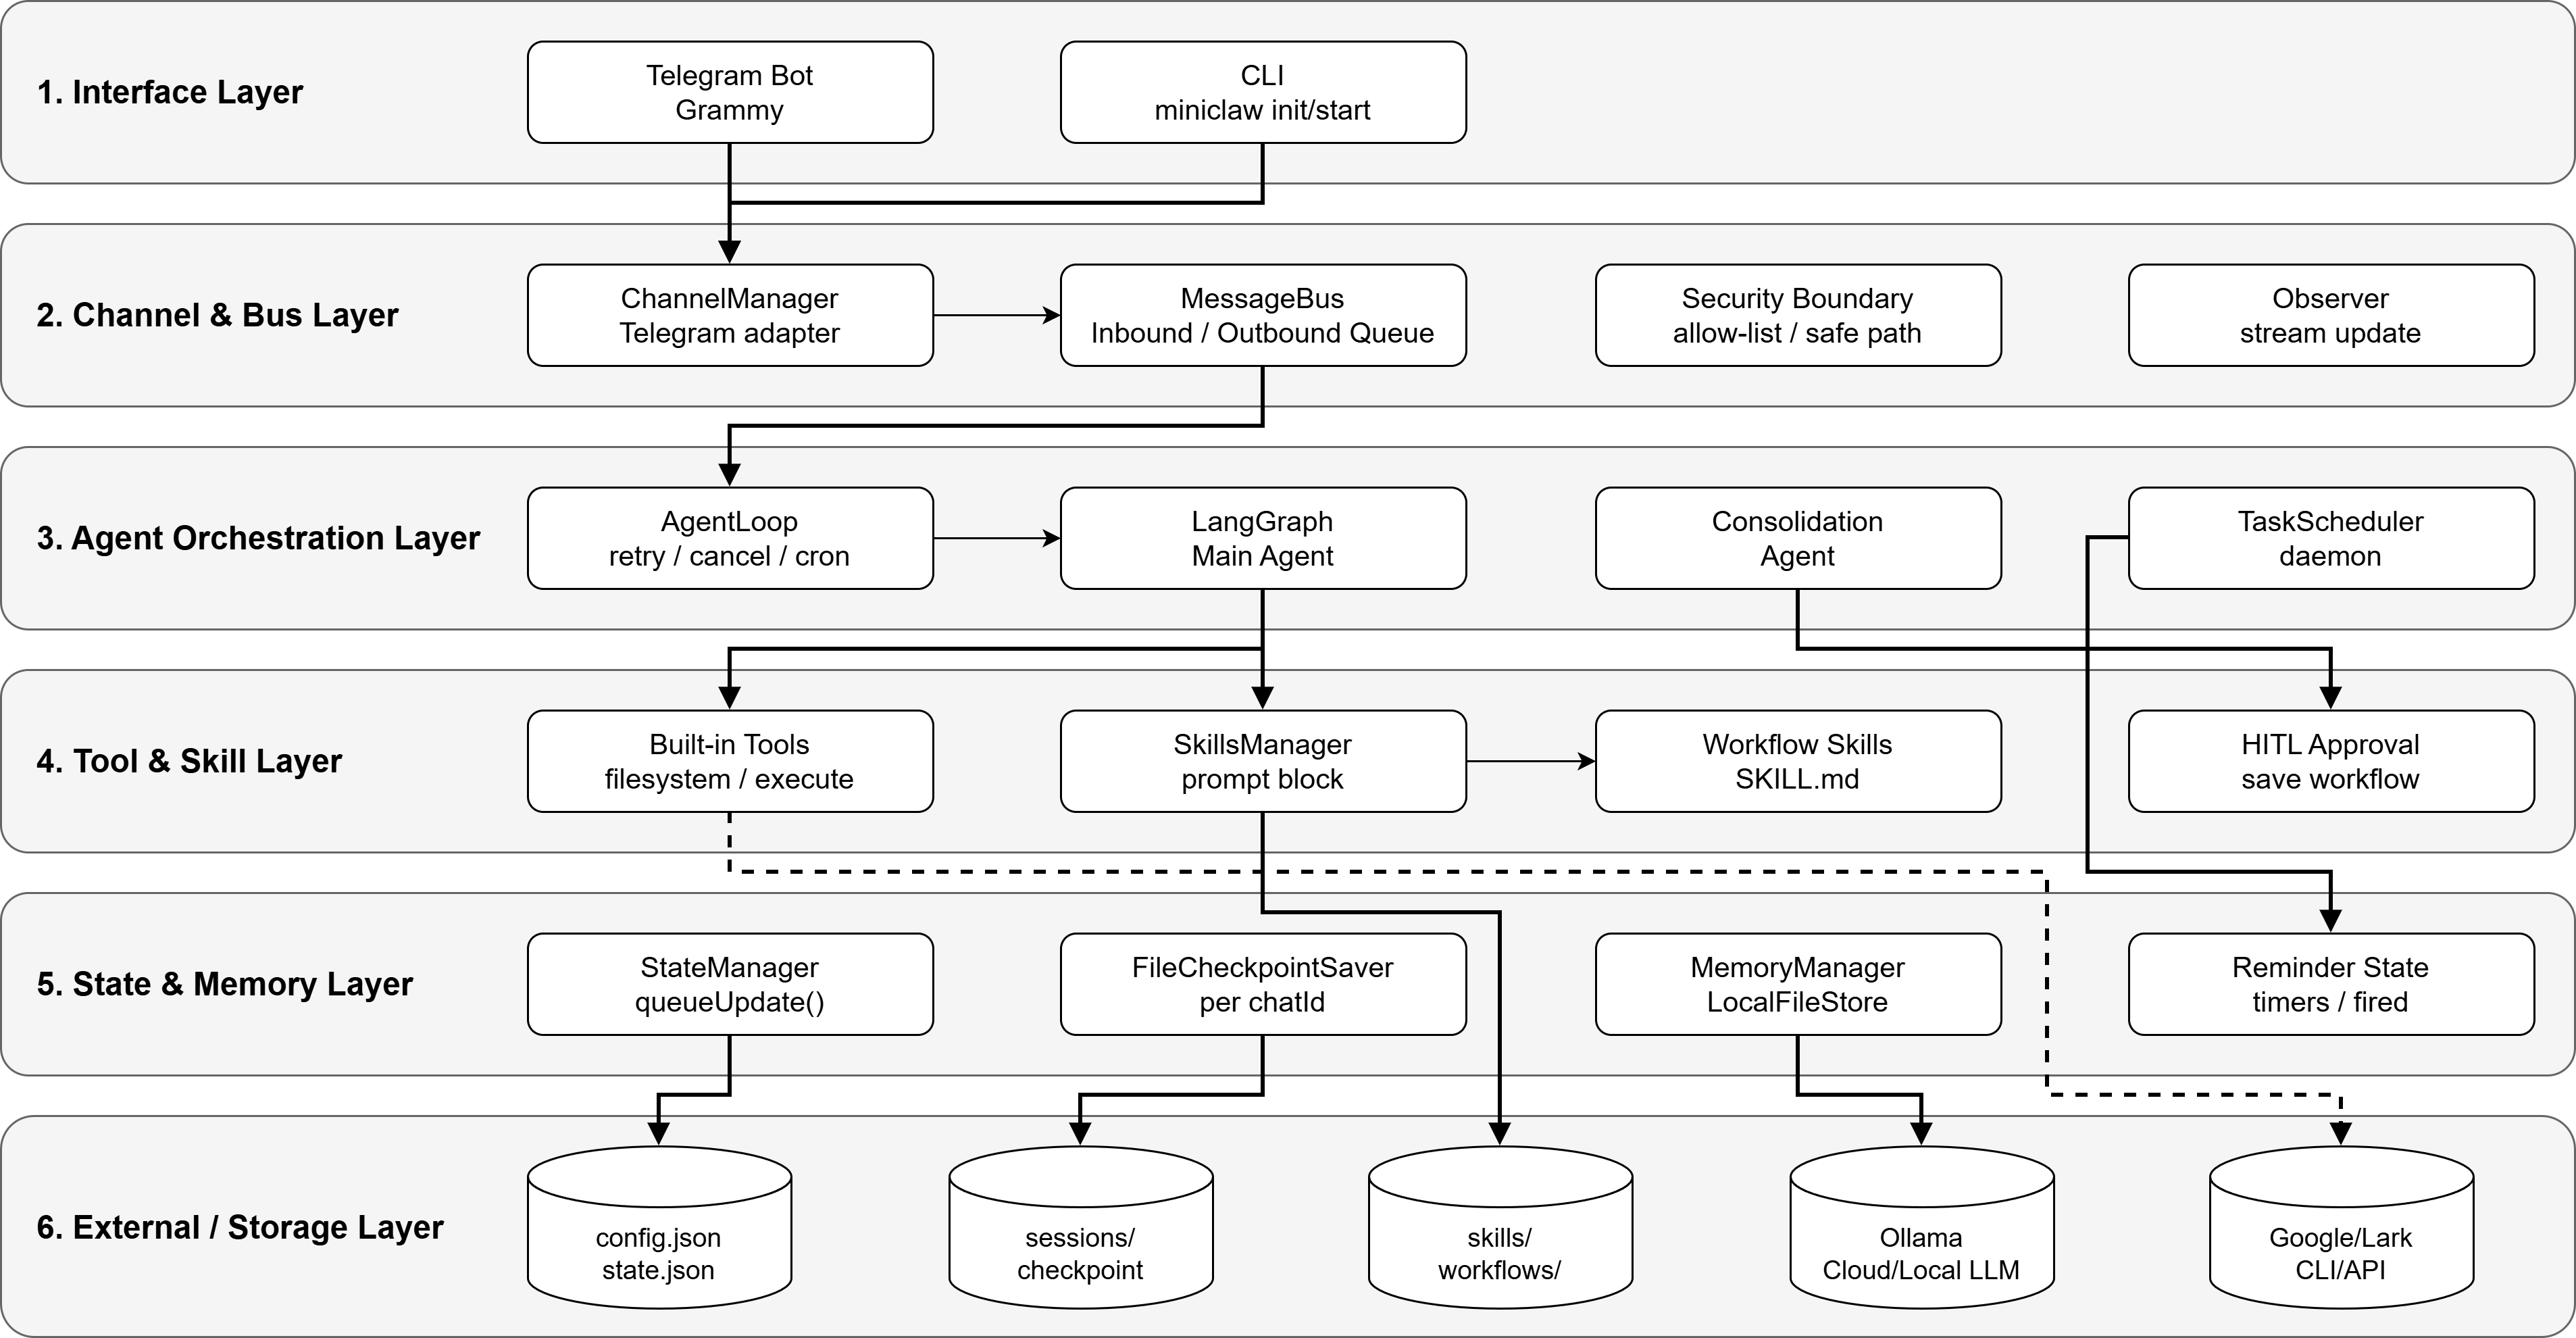
\includegraphics[width=0.96\linewidth,height=0.82\textheight,keepaspectratio]{figures/layered_architecture.drawio.png}
  \caption{\emph{Sơ đồ kiến trúc phân lớp hệ thống.}}
  \label{fig:layered-architecture}
\end{figure}
\end{landscape}
\clearpage

Hình \ref{fig:layered-architecture} nhấn mạnh quyết định tách Telegram bot khỏi lõi tác nhân. Thiết kế này làm tăng số thành phần trung gian, nhưng giúp hệ thống thay kênh giao tiếp, thay mô hình suy luận hoặc thêm kỹ năng mới mà không phá vỡ \texttt{AgentLoop}. Ranh giới bảo mật nằm trước nhóm công cụ có tác động phụ, vì vậy LLM chỉ đề xuất hành động còn runtime cục bộ mới quyết định hành động có hợp lệ hay không.

Trade-off chính của kiến trúc phân lớp nằm ở chi phí điều phối. Một yêu cầu đơn giản phải đi qua channel, bus, agent, tool và state manager trước khi trả lời người dùng. MiniClaw chấp nhận chi phí này để đổi lấy khả năng kiểm soát side-effect, quan sát lỗi tốt hơn và dễ mở rộng sang kênh giao tiếp khác.

\subsection{Cơ chế phân vùng dữ liệu và xử lý đồng thời}
MiniClaw chạy nhiều luồng bất đồng bộ trong cùng một tiến trình Node.js: tiếp nhận tin nhắn, xử lý agent, gửi nhắc nhở, cập nhật streaming message và nén ngữ cảnh. Các luồng này có tốc độ khác nhau và cùng đọc ghi một số vùng trạng thái chung. Nếu hệ thống ghi trực tiếp vào tệp JSON ở từng module, các thao tác read-modify-write có thể ghi đè lẫn nhau.

Thiết kế hiện tại xử lý vấn đề này bằng hai nguyên tắc. Thứ nhất, lịch sử hội thoại nằm trong checkpoint riêng theo \texttt{chatId}, vì vậy các phiên chat không chia sẻ cùng một tệp checkpoint. Thứ hai, trạng thái ứng dụng như active request, stream buffer, skill usage và consolidation state đi qua \texttt{StateManager.queueUpdate()}, giúp tuần tự hóa thao tác ghi vào \texttt{state.json}.

Hình \ref{fig:concurrency-isolation} biểu diễn MiniClaw theo các lane runtime để làm rõ phần nào chạy song song và phần nào bắt buộc ghi tuần tự.

\begin{landscape}
\begin{figure}[p]
  \centering
  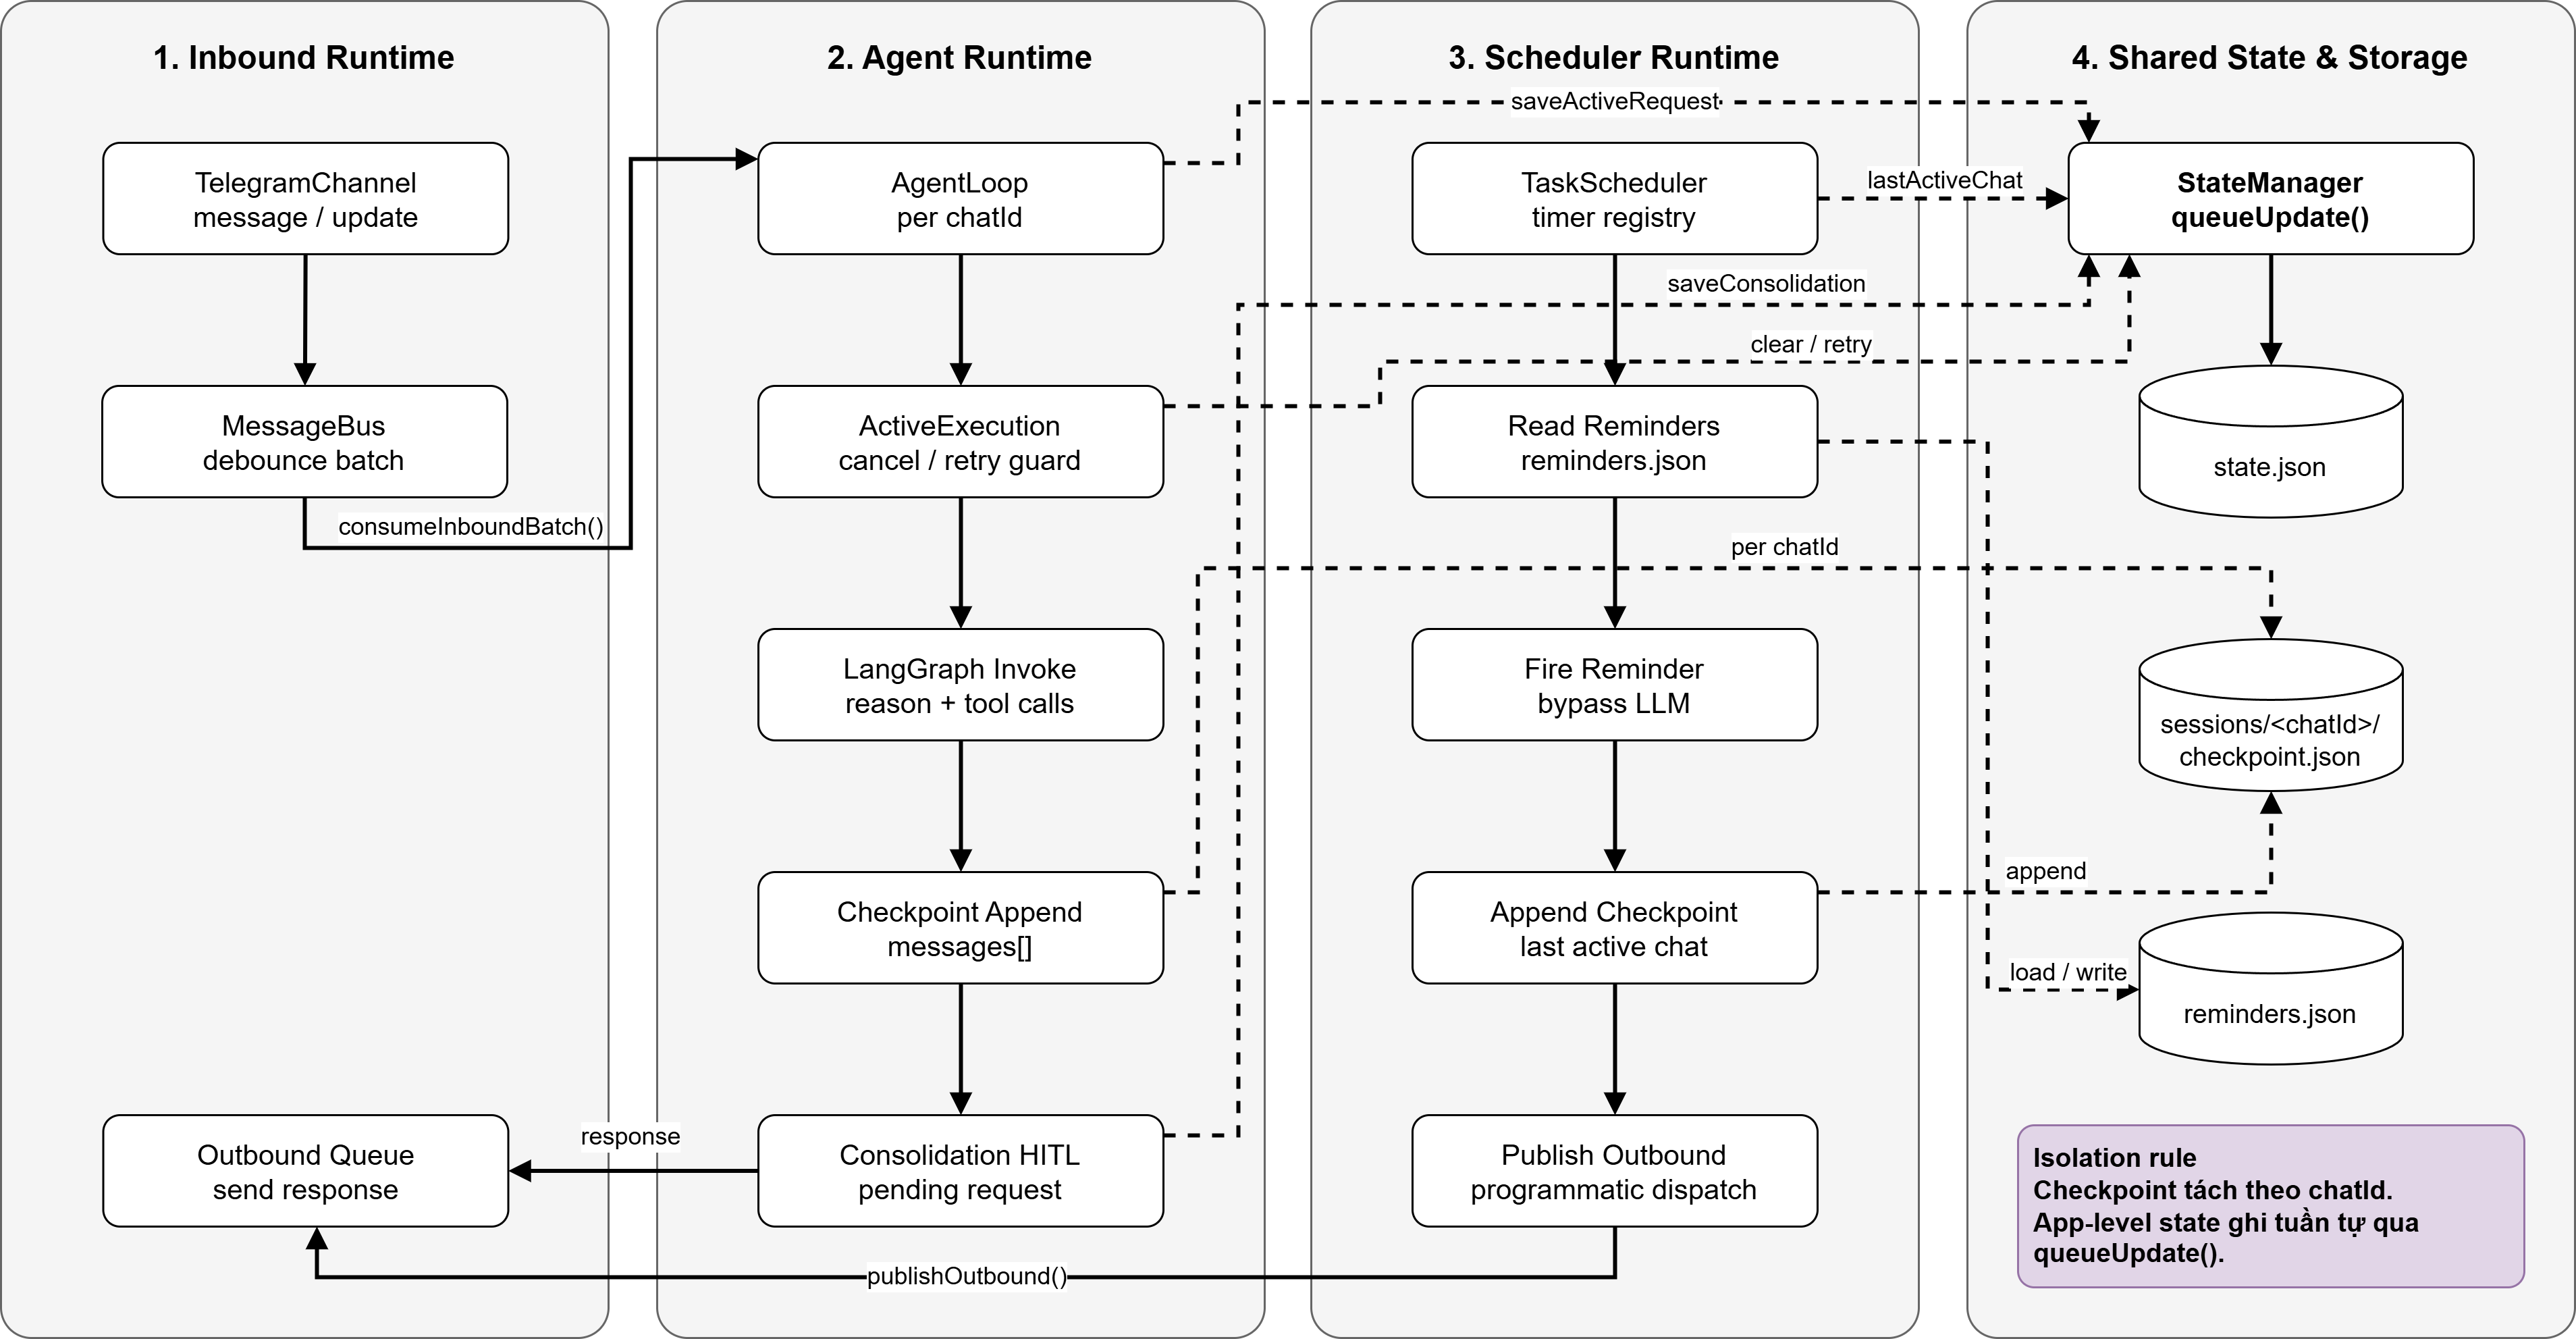
\includegraphics[width=0.96\linewidth,height=0.82\textheight,keepaspectratio]{figures/concurrency_isolation_model.drawio.png}
  \caption{\emph{Mô hình quản lý concurrency và isolation.}}
  \label{fig:concurrency-isolation}
\end{figure}
\end{landscape}
\clearpage

Hình \ref{fig:concurrency-isolation} nhấn mạnh rằng MiniClaw không xem \texttt{state.json} như cơ sở dữ liệu quan hệ, mà xem đây là vùng trạng thái ứng dụng cần ghi tuần tự. Cách tiếp cận file-based làm hệ thống gọn và dễ triển khai trong môi trường cá nhân, nhưng buộc mọi thao tác read-modify-write phải đi qua \texttt{queueUpdate()} để tránh mất cập nhật khi scheduler, Telegram stream và agent cùng ghi trạng thái. Việc tách checkpoint theo \texttt{chatId} giúp lịch sử hội thoại không trộn lẫn, đồng thời cho phép scheduler gửi nhắc nhở trực tiếp qua outbound queue mà không tiêu tốn lượt gọi LLM.

Quyết định cho scheduler bỏ qua LLM là một điểm quan trọng của kiến trúc đồng thời. Nhắc nhở đã có nội dung và thời điểm kích hoạt rõ ràng, nên gọi lại Agent chỉ làm tăng độ trễ và chi phí. Scheduler vì vậy chỉ cập nhật trạng thái, append checkpoint để giữ lịch sử nhất quán, rồi phát thông điệp ra hàng đợi outbound.

\section{Thiết kế giao diện và kịch bản tương tác}
\label{sec:ui-ux-design}

\subsection{Yêu cầu thiết kế giao diện}
Giao diện của MiniClaw được chia làm hai khu vực:
\begin{itemize}
  \item Giao diện hội thoại qua Telegram: là kênh tương tác chính của người dùng thường nhật, yêu cầu phản hồi ngắn gọn, dễ xác nhận và đủ rõ khi hệ thống gọi công cụ hoặc từ chối thao tác.
  \item Giao diện dòng lệnh (CLI): phục vụ cấu hình, onboarding và khởi tạo hệ thống cho nhà phát triển hoặc người dùng có khả năng thao tác terminal.
\end{itemize}

\subsection{Sơ đồ luồng màn hình và tương tác}
Luồng tương tác của MiniClaw bắt đầu từ CLI để khởi tạo cấu hình, sau đó chuyển sang Telegram cho các thao tác thường nhật. Trong Telegram, người dùng có thể đi qua bốn trạng thái chính: kiểm tra bot bằng lệnh hệ thống, gửi yêu cầu nghiệp vụ tự nhiên, theo dõi phản hồi khi Agent gọi công cụ, và phản hồi các lựa chọn HITL khi hệ thống đề xuất lưu workflow mới. Nếu yêu cầu vi phạm ranh giới an toàn, luồng tương tác kết thúc bằng thông báo từ chối thay vì thực thi.

\subsection{Chi tiết các kịch bản tương tác người dùng}
\subsubsection{Giao diện khởi động và cấu hình ban đầu}
Ảnh chụp màn hình thể hiện kịch bản khởi chạy onboarding thông qua lệnh \texttt{npm run dev -- init} trong terminal.

\begin{figure}[H]
  \centering
  
\includegraphics[width=0.86\linewidth]{init-terminal.png}
  \caption{\emph{Ảnh chụp giao diện chạy lệnh \texttt{npm run dev -- init}.}}
  \label{fig:screenshot-cli-init}
\end{figure}

Hình \ref{fig:screenshot-cli-init} cho thấy CLI đóng vai trò onboarding thay vì giao diện sử dụng hằng ngày. Cách tách này giúp phần cấu hình ban đầu diễn ra rõ ràng trong terminal, còn các tương tác nghiệp vụ được giữ trong Telegram.

\subsubsection{Giao diện hội thoại Telegram thường nhật}
Minh họa kịch bản trò chuyện thường nhật, trong đó người dùng kiểm tra trạng thái bot, tạo nhắc nhở hoặc yêu cầu Agent thao tác với lịch và công việc thông qua Telegram Bot.

\begin{figure}[p]
  \centering
  
\includegraphics[height=0.72\textheight]{telegram-status-and-help.png}
  \caption{\emph{Ảnh chụp Telegram khi gọi \texttt{/status} hoặc \texttt{/help}.}}
  \label{fig:screenshot-telegram-status}
\end{figure}

\begin{figure}[p]
  \centering
  
\includegraphics[height=0.72\textheight]{telegram-reminder.png}
  \caption{\emph{Ảnh chụp Telegram khi tạo nhắc nhở bằng ngôn ngữ tự nhiên.}}
  \label{fig:screenshot-telegram-reminder}
\end{figure}

\begin{figure}[p]
  \centering
  
\includegraphics[height=0.72\textheight]{telegram-calendar-task.png}
  \caption{\emph{Ảnh chụp Telegram khi MiniClaw gọi công cụ Google Workspace hoặc Lark.}}
  \label{fig:screenshot-telegram-calendar-task}
\end{figure}

Các hình \ref{fig:screenshot-telegram-status}, \ref{fig:screenshot-telegram-reminder} và \ref{fig:screenshot-telegram-calendar-task} thể hiện ba mức tương tác tăng dần. Lệnh \texttt{/status} hoặc \texttt{/help} xác nhận bot đã hoạt động, yêu cầu nhắc nhở kiểm tra đường đi Agent--Scheduler, còn yêu cầu lịch/task cho thấy giao diện Telegram vẫn giữ được tính hội thoại dù phía sau Agent đang đọc skill và gọi CLI ngoài.

\subsubsection{Giao diện nén ngữ cảnh}
Khi lịch sử hội thoại dài, người dùng có thể kích hoạt nén ngữ cảnh để MiniClaw tóm lược thông tin quan trọng và giảm kích thước checkpoint phục vụ các lượt suy luận sau.

\begin{figure}[p]
  \centering
  
\includegraphics[height=0.72\textheight]{telegram-compaction.png}
  \caption{\emph{Ảnh chụp Telegram khi kích hoạt nén ngữ cảnh bằng \texttt{/compact}.}}
  \label{fig:screenshot-telegram-compaction}
\end{figure}

Hình \ref{fig:screenshot-telegram-compaction} cho thấy cơ chế nén được trình bày như một thao tác hội thoại bình thường thay vì bắt người dùng mở file checkpoint. Đây là lựa chọn phù hợp với trợ lý cá nhân vì người dùng chỉ cần biết hệ thống đã xử lý xong và có thể tiếp tục cuộc trò chuyện.

\subsubsection{Giao diện trích xuất và phê duyệt quy trình}
Kịch bản tương tác khi hệ thống kích hoạt đề xuất trích xuất và hiển thị khung chọn kèm nút phản hồi đồng ý/hủy/sửa đổi quy trình làm việc mới.

\begin{figure}[p]
  \centering
  
\includegraphics[height=0.72\textheight]{telegram-compaction-hitl.png}
  \caption{\emph{Ảnh chụp giao diện đề xuất trích xuất và lưu quy trình.}}
  \label{fig:screenshot-extraction-prompt}
\end{figure}

Hình \ref{fig:screenshot-extraction-prompt} minh họa điểm khác biệt giữa phản hồi hội thoại thông thường và phản hồi cần phê duyệt. Workflow mới không được lưu tự động; giao diện buộc người dùng xác nhận trước khi năng lực mới đi vào thư viện kỹ năng.

\subsubsection{Giao diện cảnh báo ranh giới bảo mật}
Kịch bản bot Telegram gửi tin nhắn cảnh báo từ chối thực thi khi phát hiện lệnh nằm ngoài whitelist hoặc đường dẫn tệp tin vi phạm an toàn ranh giới.

\begin{figure}[p]
  \centering
  
\includegraphics[height=0.72\textheight]{telegram-security-deny.png}
  \caption{\emph{Ảnh chụp giao diện cảnh báo vi phạm bảo mật.}}
  \label{fig:screenshot-security-alert}
\end{figure}

Hình \ref{fig:screenshot-security-alert} thể hiện nguyên tắc thiết kế quan trọng của MiniClaw: khi không thể thực thi an toàn, giao diện phải phản hồi rõ ràng rằng yêu cầu đã bị chặn. Thông báo từ chối giúp người dùng hiểu ranh giới hệ thống mà không để Agent tạo side-effect ngoài ý muốn.
